
  \chapter{Surface Integrals}\label{chrSurf}%endchapter
   \label{chapter:surface}


 In this chapter we restrict our study to the case of surfaces in three-dimensional space. Similar results for manifolds in the n-dimensional space are presented in the chapter \ref{ch:integralofforms}.


\section{The Fundamental Vector Product}
\begin{df}

A \negrito{parametrized surface}  is given by a one-to-one
transformation $\vector{r}:\Omega \to \bbR^n$, where $\Omega$ is a domain in the
plane $\bbR^2$.  This amounts to being given three scalar functions,
$x=x(u,v)$, $y=y(u,v)$ and $z=z(u,v)$  of two variables, $u$ and
$v$, say. The transformation is then given by
$$
\vector{r}(u,v)= (x(u,v),y(u,v),z(u,v)).
$$
\end{df}


\begin{figure}[h!]
 \begin{center}
  \begin{tikzpicture}
   \usetikzlibrary{arrows}
   \draw [black!60,line width=0.3pt,-latex] (0,0) -- (4.5,0);
   \draw [black!60,line width=0.3pt,-latex] (0,0) -- (0,4.5);
   \pgfputat{\pgfpointxyz{4.4}{0.2}{0}}{\pgfbox[center,center]{\small $u$}}
   \pgfputat{\pgfpointxyz{0.2}{4.4}{0}}{\pgfbox[center,center]{\small $v$}}
   \filldraw [black,line width=1.2pt,fill=black!10] (1,1) -- (1,4) -- (4,4) --
(4,1) -- (1,1);
   \draw (1,2) -- (4,2);
   \draw (1,3) -- (4,3);
   \draw (2,1) -- (2,4);
   \draw (3,1) -- (3,4);
   \node at (2.5,2.5) {\small $\Omega$};
   \node at (2.2,4.5) {\small $\bbR^2$};
   \node [below] at (2,2) {\small $(u,v)$};
   \fill (2,2) circle (2pt);
   \shadedraw [line width=1.2pt,opacity=0.3,ball color=blue!70] (7.5,2.55)
to[out=-20,in=110] (9.7,1.55) -- (10.7,2.55)
    to[out=110,in=-20] (8.5,3.55) -- (7.5,2.55);
   \draw (7.8,2.85) to[out=-20,in=110] (10,1.85);
   \draw (8.2,3.25) to[out=-20,in=110] (10.4,2.25);
   \draw (9.3,3.35) -- (8.3,2.35);
   \draw (10,3.2) -- (9,2.2);
   \draw [black!60,line width=0.3pt,-latex] (8,1) -- (11.2,1,0);
   \draw [black!60,line width=0.3pt,-latex] (8,1) -- (8,4,0);
   \draw [black!60,line width=0.3pt,-latex] (8,1) -- (8,1,2.5);
   \pgfputat{\pgfpointxyz{11.1}{1.2}{0}}{\pgfbox[center,center]{\small $y$}};
   \pgfputat{\pgfpointxyz{8.2}{3.9}{0}}{\pgfbox[center,center]{\small $z$}};
   \pgfputat{\pgfpointxyz{8.2}{1}{2.3}}{\pgfbox[center,center]{\small $x$}};
   \pgfputat{\pgfpointxyz{8.05}{0.8}{0}}{\pgfbox[center,center]{\small $0$}};
   \node [below] at (10.3,3.6) {\small $\superficie$};
   \fill (9,3.05) circle (2pt);
   \draw [black,line width=1.2pt,-latex] (8,1) -- (8.975,3);
   \node [below right] at (8.43,1.95) {\small $\vector{r}(u,v)$};
   \draw [line width=1.5pt,-latex]  (4.5,2.7) to[out=30,in=150] (6.5,2.7);
   \node [below] at (5.5,2.7) {\small $x=x(u,v)$};
   \node [below] at (5.5,2.3) {\small $y=y(u,v)$};
   \node [below] at (5.5,1.9) {\small $z=z(u,v)$};
  \end{tikzpicture}\vspace{-4mm}
 \end{center}
 \caption[]{\quad Parametrization of a surface $\superficie$ in $\Real{3}$}
 \label{fig:surfparam}
\end{figure}\vspace{-2mm}

% Since $\funvect{r}$ is a function of two variables, we can take two partial
% derivatives: $\partial_u \funvect{r}$, the partial of $r$ with respect to $u$, and $%
% \partial_v \funvect{r}$, the partial with respect to $v$.

\begin{df} \mbox{}
\begin{itemize}
 \item  A parametrization is said \negrito{regular} at the point $(u_0,v_0)$ in $\Omega$ if
\[
\partial_u \funvect{r}(u_0,v_0)\times \partial_v \funvect{r}(u_0,v_0)\ne \vector{0}.
\]
\item The parametrization is regular if its regular for all points in $\Omega$.
\item A surface that admits a regular parametrization is said \negrito{regular parametrized surface}.
\end{itemize}
\end{df}

Henceforth, we will assume that all surfaces are regular parametrized surface.



Now we consider two curves in  $\superficie$. The first one $C_1$ is given by the vector function
\[
r_1(u)=\funvect{r}(u,v_0),u\in (a,b)
\]
obtained  keeping the variable  $v$ fixed at $v_0$.   The second curve $C_2$ is given by the vector function
\[
r_2(u)=\funvect{r}(u_0,v),v\in (c,d)
\]
this time we are keeping the variable  $u$ fixed at $u_0$).

Both curves pass through the point  $\funvect{r}(u_0,v_0):$

\begin{itemize}
 \item The curve $C_{{1}}$ has tangent vector $r_1^{\prime }(u_0)=\partial_u \funvect{r}(u_0,v_0)$
\item The curve $C_{{2}}$ has tangent vector $r_2^{\prime }(v_0)=\partial_v \funvect{r}(u_0,v_0).$
\end{itemize}


The cross product $ \vector{n}(u_0,v_0)=\partial_u \funvect{r}(u_0,v_0)\times \partial_v \funvect{r}^{\prime
}(u_0,v_0),$ which we have assumed to be different from zero, is thus
perpendicular to both curves at the point $\funvect{r}(u_0,v_0)$ and can be taken as
a normal vector  to the surface at that point.

We record the result as follows:

% \begin{figure}[h!]
%  \centering
%  \includegraphics[width=11cm]{./figs/volumefundamental.eps}
%  % volumefundamental.eps: 0x0 pixel, 300dpi, 0.00x0.00 cm, bb=0 -1 495 178
% \end{figure}



\begin{figure}[h!]
 \begin{center}
  \begin{tikzpicture}[scale=1.4]
   \usetikzlibrary{arrows}
   \draw [black!60,line width=0.3pt,-latex] (0,0) -- (4.5,0);
   \draw [black!60,line width=0.3pt,-latex] (0,0) -- (0,4.5);
   \pgfputat{\pgfpointxyz{4.4}{0.2}{0}}{\pgfbox[center,center]{\small $u$}}
   \pgfputat{\pgfpointxyz{0.2}{4.4}{0}}{\pgfbox[center,center]{\small $v$}}
   \filldraw [black,line width=1.2pt,fill=black!10] (1,1) -- (1,4) -- (4,4) --
(4,1) -- (1,1);
   \draw (1,2) -- (4,2);
   \draw (1,3) -- (4,3);
   \draw (2,1) -- (2,4);
   \draw (3,1) -- (3,4);
   \node at (2.5,2.5) {\small $\Omega$};
   \node at (2.2,4.5) {\small $\mathbb{R}^2$};
   \node [below] at (2,2) {\small $(u,v)$};
    \draw[<->] (2.1,3.2) -- (2.9,3.2);
    \node at (2.5,3.4) {$\Delta u$};
        \draw[<->] (3.1,2.9) -- (3.1,2.1);
    \node at (3.4,2.5) {$\Delta v$};


   \fill (2,2) circle (2pt);
   \shadedraw [line width=1.2pt,opacity=0.6,ball color=blue!70] (7.5,2.55)
to[out=-20,in=110] (9.7,1.55) -- (10.7,2.55)
    to[out=110,in=-20] (8.5,3.55) -- (7.5,2.55);
   \draw (7.8,2.85) to[out=-20,in=110] (10,1.85);
   \draw (8.2,3.25) to[out=-20,in=110] (10.4,2.25);
   \draw (9.3,3.35) -- (8.3,2.35);
   \draw (10,3.2) -- (9,2.2);
   \draw [black!60,line width=0.3pt,-latex] (8,1) -- (11.2,1,0);
   \draw [black!60,line width=0.3pt,-latex] (8,1) -- (8,4,0);
   \draw [black!60,line width=0.3pt,-latex] (8,1) -- (8,1,2.5);
%    \pgfputat{\pgfpointxyz{11.1}{1.2}{0}}{\pgfbox[center,center]{\small $y$}};
%    \pgfputat{\pgfpointxyz{8.2}{3.9}{0}}{\pgfbox[center,center]{\small $z$}};
%    \pgfputat{\pgfpointxyz{8.2}{1}{2.3}}{\pgfbox[center,center]{\small $x$}};
%    \pgfputat{\pgfpointxyz{8.05}{0.8}{0}}{\pgfbox[center,center]{\small $0$}};

   \node [below] at (10.3,3.6) {\small $\superficie$};
   \fill (8.6,2.64) circle (1pt);
     \draw[red,<->] (8.52,2.73) -- (8.88,3.074);
  \node at (8.35,3) {\small$\funvect{r}_u\Delta u$};
     \draw[red,<->] (8.6,2.53) -- (9.14,2.41);
       \node at (9.15,2.7) {\small$\funvect{r}_v\Delta v$};


   \draw [black,line width=1.2pt,-latex] (8,1) -- (8.6,2.64);
   \node [below right] at (7.,1.6) {\small $\vector{r}(u,v)$};
   \draw [line width=1.5pt,-latex]  (4.5,2.7) to[out=30,in=150] (6.5,2.7);
      \node [above] at (5.5,3) {\small $\vector{r}(u,v)$};
%    \node [below] at (5.5,2.7) {\small $x=x(u,v)$};
%    \node [below] at (5.5,2.3) {\small $y=y(u,v)$};
%    \node [below] at (5.5,1.9) {\small $z=z(u,v)$};
  \end{tikzpicture}\vspace{-4mm}
 \end{center}
 \caption[]{\quad Parametrization of a surface $\superficie$ in $\mathbb{R}^3$}
 \label{fig:surfparam}
\end{figure}


\begin{df}
 If $\superficie$ is a regular surface given by a differentiable function $\funvect{r}=\funvect{r}(u,v),$ then the cross product
\[\vector{n}(u,v)=\partial_u \funvect{r}\times \partial_v \funvect{r}\]
is called the \negrito{fundamental vector product} of the surface.
\end{df}





\begin{exa}
  For the plane $\funvect{r}(u,v)=u\vector{a}+v\vector{b}+\vector{c}$ we have

$\partial_u \funvect{r}(u,v)=\vector{a}$, $\partial_v \funvect{r}(u,v)=\vector{b}$ and therefore $\hat{ \vector{n}}(u,v)=\vector{a}\times
\vector{b}$. The vector $\vector{a}\times \vector{b}$ is normal to the plane.
\end{exa}


\begin{exa}
We parametrized the sphere $x^2+y^2+z^2=a^2$ by setting
\[
\funvect{r}(u,v)=a\cos \,u\sin \,v\vector{i}+a\sin \,u\sin \,v\vector{j}+a\cos \,v\vector{k},
\]
with $0\le u\le 2\pi ,0\le v\le \pi .$ In this case
\[
\partial_u \funvect{r}(u,v)=-a\sin u\sin v\vector{i}+a\cos u\sin v\vector{j}
\]
and
\[
\partial_v \funvect{r}(u,v)=a\cos \,u\cos \,v\vector{i}+a\sin u\cos v\vector{j}-a\sin v\vector{k}.
\]
Thus
\[
 \vector{n}(u,v)=\left|
\begin{array}{ccc}
\vector{i} & \vector{j} & \vector{k} \\
-a\sin u\cos v & a\cos u\cos v & 0 \\
a\cos \,u\cos \,v & a\sin u\cos v & a\sin v
\end{array}
\right|
\]
\[
=-a \sin v  \left(  a\cos \,u\sin \,v\vector{i}+a\sin \,u\sin \,v\vector{j}+a\cos \,v\vector{k},   \right) \]
\[
=a\sin \,v\,\funvect{r}(u,v).
\]
As was to be expected, the fundamental vector product of a sphere is
parallel to the radius vector $\funvect{r}(u,v).$


\begin{exa}\leavevmode
  \begin{enumerate}
    \item Take the sphere $f(\vector{r}) = x^2 + y^2 + z^2 = c$ for $c > 0$. Then $\nabla f = 2(x, y, z) = 2\vector{r}$, which is clearly normal to the sphere.
    \item Take $f(\vector{r}) = x^2 + y^2 - z^2 = c$, which is a hyperboloid. Then $\nabla f = 2(x, y, -z)$.

      In the special case where $c = 0$, we have a double cone, with a singular apex $\vector{0}$. Here $\nabla f = \vector{0}$, and we cannot find a meaningful direction of normal.
  \end{enumerate}
\end{exa}

\begin{definition}[Boundary]
  A surface $\superficie$ can have a \negrito{boundary} $\partial \superficie$. We are interested in the case where the boundary  consist of a piecewise smooth curve or in a union of piecewise smooth curves. 

  A surface is \negrito{bounded} if it can be contained in a solid sphere of radius $R$, and is called  \emph{unbounded} otherwise. A bounded surface with no boundary is called \negrito{closed}.
\end{definition}


\begin{exa}
  The boundary of a hemisphere is a circle (drawn in red).
\leavevmode
  \begin{center}
    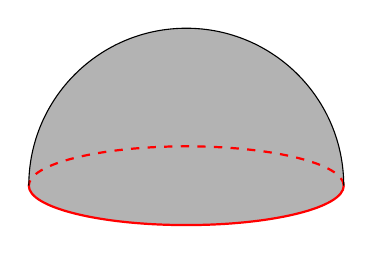
\begin{tikzpicture}
      \draw [draw=none, fill=gray, opacity=0.6] (-2, 0) arc (180:360:2 and 0.5) arc (0:180:2);
      \draw [red, thick, dashed] (2, 0) arc (0:180:2 and 0.5);
      \draw [red, thick] (-2, 0) arc (180:360:2 and 0.5);
      \draw (2, 0) arc (0:180:2);
    \end{tikzpicture}
  \end{center}
\end{exa}

\begin{exa} The sphere and the torus are examples of closed surfaces. Both are bounded and without boundaries.
\end{exa}
%
% \begin{definition}[Orientable surface]
%   At each point, there is a unit normal $\hat{\vector{n}}$ that's unique up to a sign.
%
%   If we can find a consistent choice of $\hat{\vector{n}}$ that varies smoothly across $S$, then we say $S$ is \negrito{orientable}, and the choice of sign of $\hat{\vector{n}}$ is called the \negrito{orientation} of the surface.
% \end{definition}
% Most surfaces we encounter are orientable. For example, for a sphere, we can declare that the normal should always point outwards. A notable example of a non-orientable surface is the M\"obius strip (or Klein bottle).
%
% For simple cases, we can describe the orientation as ``inward'' and ``outward''.




\end{exa}

\section{The Area of a Parametrized Surface}


We will now learn how to perform integration over a
\emph{surface} in $\Real{3}$.\index{integral!surface}\index{surface integral}


Similar to how we used a parametrization of a curve to define the line integral along the curve, we will use a
parametrization of a surface to define a \emph{surface integral}. We will use \emph{two} variables, $u$ and $v$,
to parametrize a surface $\superficie$ in $\Real{3}$: $x=x(u,v)$, $y=y(u,v)$, $z=z(u,v)$, for $(u,v)$ in some region $\Omega$ in
$\Real{2}$ (see Figure \ref{fig:surfparam}).



\begin{figure}[h!]
 \begin{center}
  \begin{tikzpicture}[scale=1.4]
   \usetikzlibrary{arrows}
   \draw [black!60,line width=0.3pt,-latex] (0,0) -- (4.5,0);
   \draw [black!60,line width=0.3pt,-latex] (0,0) -- (0,4.5);
   \pgfputat{\pgfpointxyz{4.4}{0.2}{0}}{\pgfbox[center,center]{\small $u$}}
   \pgfputat{\pgfpointxyz{0.2}{4.4}{0}}{\pgfbox[center,center]{\small $v$}}
   \filldraw [black,line width=1.2pt,fill=black!10] (1,1) -- (1,4) -- (4,4) --
(4,1) -- (1,1);
   \draw (1,2) -- (4,2);
   \draw (1,3) -- (4,3);
   \draw (2,1) -- (2,4);
   \draw (3,1) -- (3,4);
   \node at (2.5,2.5) {\small $\Omega$};
   \node at (2.2,4.5) {\small $\mathbb{R}^2$};
   \node [below] at (2,2) {\small $(u,v)$};
    \draw[<->] (2.1,3.2) -- (2.9,3.2);
    \node at (2.5,3.4) {$\Delta u$};
        \draw[<->] (3.1,2.9) -- (3.1,2.1);
    \node at (3.4,2.5) {$\Delta v$};


   \fill (2,2) circle (2pt);
   \shadedraw [line width=1.2pt,opacity=0.6,ball color=blue!70] (7.5,2.55)
to[out=-20,in=110] (9.7,1.55) -- (10.7,2.55)
    to[out=110,in=-20] (8.5,3.55) -- (7.5,2.55);
   \draw (7.8,2.85) to[out=-20,in=110] (10,1.85);
   \draw (8.2,3.25) to[out=-20,in=110] (10.4,2.25);
   \draw (9.3,3.35) -- (8.3,2.35);
   \draw (10,3.2) -- (9,2.2);
   \draw [black!60,line width=0.3pt,-latex] (8,1) -- (11.2,1,0);
   \draw [black!60,line width=0.3pt,-latex] (8,1) -- (8,4,0);
   \draw [black!60,line width=0.3pt,-latex] (8,1) -- (8,1,2.5);
%    \pgfputat{\pgfpointxyz{11.1}{1.2}{0}}{\pgfbox[center,center]{\small $y$}};
%    \pgfputat{\pgfpointxyz{8.2}{3.9}{0}}{\pgfbox[center,center]{\small $z$}};
%    \pgfputat{\pgfpointxyz{8.2}{1}{2.3}}{\pgfbox[center,center]{\small $x$}};
%    \pgfputat{\pgfpointxyz{8.05}{0.8}{0}}{\pgfbox[center,center]{\small $0$}};

   \node [below] at (10.3,3.6) {\small $\superficie$};
   \fill (8.6,2.64) circle (1pt);
     \draw[red,<->] (8.52,2.73) -- (8.88,3.074);
  \node at (8.35,3) {\small$\funvect{r}_u\Delta u$};
     \draw[red,<->] (8.6,2.53) -- (9.14,2.41);
       \node at (9.15,2.7) {\small$\funvect{r}_v\Delta v$};


   \draw [black,line width=1.2pt,-latex] (8,1) -- (8.6,2.64);
   \node [below right] at (7.,1.6) {\small $\vector{r}(u,v)$};
   \draw [line width=1.5pt,-latex]  (4.5,2.7) to[out=30,in=150] (6.5,2.7);
      \node [above] at (5.5,3) {\small $\vector{r}(u,v)$};
%    \node [below] at (5.5,2.7) {\small $x=x(u,v)$};
%    \node [below] at (5.5,2.3) {\small $y=y(u,v)$};
%    \node [below] at (5.5,1.9) {\small $z=z(u,v)$};
  \end{tikzpicture}\vspace{-4mm}
 \end{center}
 \caption[]{\quad Parametrization of a surface $\superficie$ in $\mathbb{R}^3$}
 \label{fig:surfparam}
\end{figure}

In this case, the position vector of a point on the surface $\superficie$ is given by the vector-valued function
\begin{displaymath}
 \vector{r}(u,v) ~=~ x(u,v) \vector{i} ~+~ y(u,v) \vector{j} ~+~ z(u,v) \vector{k} ~~\text{for $(u,v)$ in $\Omega$.}
\end{displaymath}

% Since $\vector{r}(u,v)$ is a function of two variables, define the partial derivatives
% $\dfrac{\partial \vector{r}}{\partial u}$ and $\dfrac{\partial \vector{r}}{\partial v}$ for $(u,v)$ in $\Omega$ by
% \begin{align*}
%  \dfrac{\partial \vector{r}}{\partial u}(u,v) ~&=~
%  \dfrac{\partial x}{\partial u}(u,v) \vector{i} ~+~ \dfrac{\partial y}{\partial u}(u,v) \vector{j} ~+~
%  \dfrac{\partial z}{\partial u}(u,v) \vector{k} ~,~~\text{and}\vspace{1mm}\\
%  \dfrac{\partial \vector{r}}{\partial v}(u,v) ~&=~
%  \dfrac{\partial x}{\partial v}(u,v) \vector{i} ~+~ \dfrac{\partial y}{\partial v}(u,v) \vector{j} ~+~
%  \dfrac{\partial z}{\partial v}(u,v) \vector{k} ~.
% \end{align*}

The parametrization of $\superficie$ can be thought of as ``transforming'' a region in $\Real{2}$ (in the $uv$-plane) into
a 2-dimensional surface in $\Real{3}$. This parametrization of the surface is sometimes called a \emph{patch}, based
on the idea of ``patching'' the region $\Omega$ onto $\superficie$ in the grid-like manner shown in Figure \ref{fig:surfparam}.

In fact, those gridlines in $\Omega$ lead us to how we will define a surface integral over $\superficie$. Along the
vertical gridlines in $\Omega$, the variable $u$ is constant. So those lines get mapped to curves on $\superficie$, and the
variable $u$ is constant along the position vector $\vector{r}(u,v)$. Thus, the tangent vector to those curves at a
point $(u,v)$ is $\dfrac{\partial \vector{r}}{\partial v}$. Similarly, the horizontal gridlines in $\Omega$ get mapped to
curves on $\superficie$ whose tangent vectors are $\dfrac{\partial \vector{r}}{\partial u}$.


\begin{center}
\vspace{0.7cm}
\begin{overpic}[width=11cm, tics=10]{./figs/parametrized_surface_mapping_labeled.eps}
    \put (-5,-5) {$(u,v)$}
    \put (-5,25) {$(u,v+\Delta v)$}
    \put (24,-5) {$(u +\Delta u,v)$}
    \put (24,25) {$(u +\Delta u,v+\Delta v)$}

        \put (80,-5) {$r(u,v)$}
        \put (55,18) {$r(u,v+\Delta v))$}
        \put (103,10) {$r(u+\Delta u,v))$}


%   \put (53,2) {$\caminho$}
 \end{overpic}
 \vspace{0.7cm}
 \end{center}



Now take a point $(u,v)$ in $\Omega$ as, say,
the lower left corner of one of the rectangular grid sections in $\Omega$, as shown in Figure \ref{fig:surfparam}. Suppose
that this rectangle has a small width and height of $\Delta u$ and $\Delta v$, respectively. The corner points of that
rectangle are $(u,v)$, $(u+\Delta u,v)$, $(u+\Delta u,v+\Delta v)$ and $(u,v+\Delta v)$.
So the area of that
rectangle is $A = \Delta u\,\Delta v$. Then that rectangle gets mapped by the parametrization onto some section of the
surface $\superficie$ which, for $\Delta u$ and $\Delta v$ small enough, will have a surface area (call it $ \d \S$) that
is very close to the area of the parallelogram which has adjacent sides $\vector{r}(u+\Delta u,v) - \vector{r}(u,v)$
(corresponding to the line segment from $(u,v)$ to $(u+\Delta u,v)$ in $\Omega$) and
$\vector{r}(u,v+\Delta v) - \vector{r}(u,v)$ (corresponding to the line segment from $(u,v)$ to $(u,v+\Delta v)$ in
$\Omega$). But by combining our usual notion of a partial derivative  with that of the derivative of a vector-valued function  applied to a function of two variables, we have
\begin{align*}
 \dfrac{\partial \vector{r}}{\partial u} ~&\approx~ \dfrac{\vector{r}(u+\Delta u,v) - \vector{r}(u,v)}{\Delta u}
 ~,~~\text{and}\vspace{1mm}\\
 \dfrac{\partial \vector{r}}{\partial v} ~&\approx~ \dfrac{\vector{r}(u,v+\Delta v) - \vector{r}(u,v)}{\Delta v} ~,
\end{align*}
and so the surface area element $ \d \S$ is approximately
\begin{displaymath}
 \Norm{\Crossprod{(\vector{r}(u+\Delta u,v) - \vector{r}(u,v))}{(\vector{r}(u,v+\Delta v) - \vector{r}(u,v))}} \approx
\Norm{\Crossprod{(\Delta u \dfrac{\partial \vector{r}}{\partial u})}{(\Delta v\dfrac{\partial \vector{r}}{\partial v})}}
 =\Norm{\Crossprod{\dfrac{\partial \vector{r}}{\partial u}}{\dfrac{\partial \vector{r}}{\partial v}}}\,
 \Delta u \, \Delta v
\end{displaymath}

Thus, the total surface area $S$ of $\superficie$ is approximately the sum of all the quantities
$\Norm{\Crossprod{\dfrac{\partial \vector{r}}{\partial u}}{\dfrac{\partial \vector{r}}{\partial v}}}\,\Delta u\,\Delta v$,
summed over the rectangles in $\Omega$. Taking the limit of that sum as the diagonal of the largest rectangle goes to $0$
gives
\begin{equation}
 S ~=~ \diint\limits_{\Omega}\,\Norm{\Crossprod{\dfrac{\partial \vector{r}}{\partial u}}{\dfrac{\partial \vector{r}}{\partial v}}}
 \,du\,dv ~.
\end{equation}
We will write the double integral on the right using the special notation
\begin{equation}
 \diint\limits_{\superficie}  \d \S ~=~
 \diint\limits_{\Omega}\,\NORM{\Crossprod{\dfrac{\partial \vector{r}}{\partial u}}{\dfrac{\partial \vector{r}}{\partial v}}}
 \,du\,dv ~.
\end{equation}
This is a special case of a \emph{surface integral} over the surface $\superficie$, where the surface area element
$\d \S$ can be thought of as $1\,\d \S$. Replacing $1$ by a general real-valued function $f(x,y,z)$ defined
in $\Real{3}$, we have the following:

\begin{df}
\label{defn:surfintreal}
 Let $\superficie$ be a surface in $\Real{3}$ parametrized by
 \[x=x(u,v), \quad y=y(u,v), \quad z=z(u,v),\] for $(u,v)$ in some
  region $\Omega$ in $\Real{2}$. Let $\vector{r}(u,v) = x(u,v) \vector{i} + y(u,v) \vector{j} + z(u,v) \vector{k}$ be the
  position vector for any point on $\superficie$. The surface area $S$ of $\superficie$ is defined as \index{integral!surface}\index{surface integral}
  \begin{equation}
   S ~=~ \diint\limits_{\superficie} 1\,\d \S ~=~ \diint\limits_{\Omega}
  \Norm{\Crossprod{\dfrac{\partial \vector{r}}{\partial u}}{\dfrac{\partial \vector{r}}{\partial v}}}\,du\,dv
  \end{equation}
  \end{df}

\begin{exa}
 A \emph{torus} $T$ is a surface obtained by revolving a circle of radius $a$ in the $yz$-plane around the $z$-axis,
 where the circle's center is at a distance $b$ from the z-axis ($0<a<b$), as in Figure \ref{fig:torus}. Find the
 surface area of $T$.\index{torus}

 \begin{figure}[h!]
 \centering
 \subfloat[][Circle in the $yz$-plane]{
 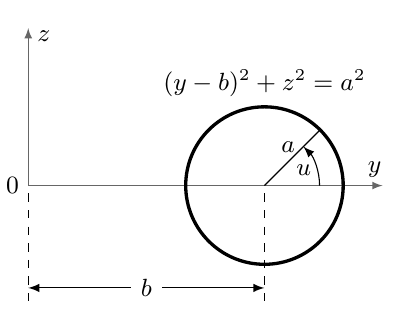
\begin{tikzpicture}
  \usetikzlibrary{arrows}
  \draw [black!60,line width=0.3pt,-latex] (0,0) -- (4.5,0);
  \draw [black!60,line width=0.3pt,-latex] (0,0) -- (0,2);
  \pgfputat{\pgfpointxyz{4.4}{0.2}{0}}{\pgfbox[center,center]{\small $y$}}
  \pgfputat{\pgfpointxyz{0.2}{1.9}{0}}{\pgfbox[center,center]{\small $z$}}
  \pgfputat{\pgfpointxyz{-0.2}{0}{0}}{\pgfbox[center,center]{\small $0$}}
  \draw [line width=1.2pt] (3,0) circle (1);
  \draw (3,0) -- (3.707,0.707);
  \draw [-latex] (3.7,0) arc (0:45:0.7);
  \node [above] at (3.3,0.3) {\small $a$};
  \node [above] at (3,1) {\small $(y-b)^2 + z^2 = a^2$};
  \node at (3.5,0.2) {\small $u$};
  \draw [dashed] (0,-0.1) -- (0,-1.5);
  \draw [dashed] (3,-0.1) -- (3,-1.5);
  \node at (1.5,-1.3) {\small $b$};
  \draw [-latex] (1.7,-1.3) -- (3,-1.3);
  \draw [-latex] (1.3,-1.3) -- (0,-1.3);
 \end{tikzpicture}}
 \qquad\qquad
 \subfloat[][Torus $T$]{\includegraphics{./figs/torus.0}}
 \caption[]{}
 \label{fig:torus}
\end{figure}

\end{exa}
\begin{solu}

For any point on the circle, the line segment from the center of the circle to that point makes an angle $u$ with the
$y$-axis in the positive $y$ direction (see Figure \ref{fig:torus}(a)). And as the circle revolves around the $z$-axis,
the line segment from the origin to the center of that circle sweeps out an angle $v$ with the positive $x$-axis (see
Figure \ref{fig:torus}(b)). Thus, the torus can be parametrized as:
\begin{displaymath}
 x = (b+a\cos u)\cos v ~,\quad y = (b+a\cos u)\sin v ~,\quad z = a\sin u~,\quad 0\le u\le 2\pi~,\quad 0\le v\le 2\pi
\end{displaymath}
So for the position vector
\begin{align*}
 \vector{r}(u,v) ~&=~ x(u,v) \vector{i} ~+~ y(u,v) \vector{j} ~+~ z(u,v) \vector{k}\\
 &=~ (b+a\cos u)\cos v \,\vector{i} ~+~ (b+a\cos u)\sin v \,\vector{j} ~+~ a\sin u \,\vector{k}
\end{align*}
we see that
\begin{align*}
 \dfrac{\partial \vector{r}}{\partial u} ~&=~
  -a\sin u\,\cos v \,\vector{i} ~-~ a\sin u\,\sin v \,\vector{j} ~+~ a\cos u \,\vector{k}\\[6pt]
 \dfrac{\partial \vector{r}}{\partial v} ~&=~
  -(b+a\cos u)\sin v \,\vector{i} ~+~ (b+a\cos u)\cos v \,\vector{j} ~+~ 0 \vector{k} ~,
\end{align*}
and so computing the cross product gives
\begin{displaymath}
 \Crossprod{\dfrac{\partial \vector{r}}{\partial u}}{\dfrac{\partial \vector{r}}{\partial v}} ~=~
  -a(b+a\cos u)\cos v\,\cos u \,\vector{i} ~-~ a(b+a\cos u)\sin v\,\cos u\,\vector{j} ~-~ a(b+a\cos u)\sin u \,\vector{k} ~,
\end{displaymath}
which has magnitude
\begin{displaymath}
\Norm{\Crossprod{\dfrac{\partial \vector{r}}{\partial u}}{\dfrac{\partial \vector{r}}{\partial v}}} ~=~ a(b+a\cos u) ~.
\end{displaymath}
Thus, the surface area of $T$ is
\begin{align*}
 S ~&=~ \diint\limits_{\superficie} 1\,\d \S\\[6pt]
  &=~ \dint_0^{2\pi} \dint_0^{2\pi}\,\NORM{\Crossprod{\dfrac{\partial \vector{r}}{\partial u}}{\dfrac{\partial
  \vector{r}}{\partial v}}}\,du\,dv\\[6pt]
  &=~ \dint_0^{2\pi} \dint_0^{2\pi} a(b+a\cos u)\,du\,dv\\[6pt]
  &=~ \dint_0^{2\pi} \left( abu + a^2 \sin u \,\Big|_{u=0}^{u=2\pi}\,\right)\,dv\\[6pt]
  &=~ \dint_0^{2\pi} 2\pi ab\,dv\\
  &=~ 4\pi^2 ab
\end{align*}
\end{solu}


\begin{figure}[h!]
\centering
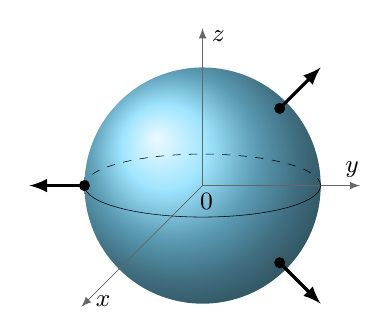
\begin{tikzpicture}
 \usetikzlibrary{arrows}
 \definecolor{spherecolor}{HTML}{80DCFF}
 \shade [ball color=spherecolor] (0,0) circle (1.5);
 \draw [black!60,line width=0.3pt,-latex] (0,0) -- (2,0,0);
 \draw [black!60,line width=0.3pt,-latex] (0,0) -- (0,2,0);
 \draw [black!60,line width=0.3pt,-latex] (0,0) -- (0,0,4);
 \pgfputat{\pgfpointxyz{1.9}{0.2}{0}}{\pgfbox[center,center]{\small $y$}};
 \pgfputat{\pgfpointxyz{0.2}{1.9}{0}}{\pgfbox[center,center]{\small $z$}};
 \pgfputat{\pgfpointxyz{0.2}{0}{3.8}}{\pgfbox[center,center]{\small $x$}};
 \pgfputat{\pgfpointxyz{0.05}{-0.2}{0}}{\pgfbox[center,center]{\small $0$}};
 \draw [line width=0.2pt] (-1.5,0) arc (180:360:1.5 and 0.4);
 \draw [dashed,line width=0.2pt] (1.5,0) arc (0:180:1.5 and 0.4);
 \fill (0.98,0.98) circle (2pt);
 \draw [line width=1.2pt,-latex] (0.98,0.98) -- (1.5,1.5);
 \fill (0.98,-0.98) circle (2pt);
 \draw [line width=1.2pt,-latex] (0.98,-0.98) -- (1.5,-1.5);
 \fill (-1.5,0) circle (2pt);
 \draw [line width=1.2pt,-latex] (-1.5,0) -- (-2.2,0);
\end{tikzpicture}
\end{figure}



\begin{exa}

[The surface area of a sphere] The function
\[
\funvect{r}(u,v)=a\cos \,u\sin \,v\vector{i}+a\sin \,u\sin \,v\vector{j}+a\cos \,v\vector{k},
\]
with $(u,v)$ ranging over the set $0\le u\le 2\pi ,0\le v\le
\dfrac \pi 2$ parametrizes a sphere of radius $a$. For this parametrization

\begin{center}
$ \vector{n}(u,v)=a\sin \,v\,\funvect{r}(u,v)$ and $\left\|  \vector{n}(u,v)\right\| =a^2\left| \sin
\,v\right| =a^2\sin \,v.$
\end{center}

So,

area of the sphere $=\diint_\Omega a^2\sin \,v\du\dv$%
\[
=\dint_0^{2\pi }\left( \dint_{0}^{ \pi }a^2\sin \,v\dv\right)
du=2\pi a^2\dint_{0}^{\pi }\sin \,v\dv=4\pi a^2,
\]
which is known to be correct.
\end{exa}

\begin{exa}[The area of a region of the plane] If $\superficie$ is a plane region $%
\Omega $, then $\superficie$ can be parametrized by setting
\[
\funvect{r}(u,v)=ui+vj,(u,v)\in \Omega .
\]
Here $ \vector{n}(u,v)=\partial_u \funvect{r}(u,v)\times \partial_v \funvect{r}(u,v)=i\times j=k$ and $%
\left\| \vector{n}(u,v)\right\| =1$. In this case we reobtain  the familiar formula
\[
A=\diint_\Omega \du\dv.
\]

\end{exa}

\begin{exa}[The area of a surface of revolution] Let $\superficie$ be the
surface generated by revolving the graph of a function
\[
y=f(x),x\in [a,b]
\]
about the $x$-axis. We will assume that $f$ is positive and continuously
differentiable.

We can parametrize $\superficie$ by setting
\[
\funvect{r}(u,v)=vi+f(v)\cos \,u\;j+f(v)\sin \,u\;k
\]
with $(u,v)$ ranging over the set $\Omega :0\leq u\leq 2\pi ,a\le v\le b.$
In this case
\[
 \vector{n}(u,v)=\partial_u \funvect{r}(u,v)\times \partial_v \funvect{r}(u,v)=\left|
\begin{array}{ccc}
i & j & k \\
0 & -f(v)\sin \,u & f(v)\cos \,u \\
1 & f^{\prime }(v)\cos \,u & f^{\prime }(v)\sin \,u
\end{array}
\right|
\]
\[
=-f(v)f^{\prime }(v)i+f(v)\cos \,u\;j+f(v)\sin \,u\;k.
\]
Therefore $\left\|\vector{n}(u,v)\right\| =f(v)\sqrt{\left[ f^{\prime }(v)\right]
^2+1}$ and

\begin{center}
$\area{\superficie}=\diint_\Omega f(v)\sqrt{\left[ f^{\prime }(v)\right] ^2+1}\,\du\dv$%
\[
\dint_0^{2\pi }\left( \dint_a^bf(v)\sqrt{\left[ f^{\prime }(v)\right] ^2+1}%
\dv\right) du=\dint_a^b2\pi f(v)\sqrt{\left[ f^{\prime }(v)\right] ^2+1}\dv.
\]
\end{center}

\end{exa}

\begin{exa}[ Spiral ramp] One turn of the spiral ramp of Example
5 is the surface
\[
\superficie:\funvect{r}(u,v)=u\cos \omega v\;\vector{i}+u\sin \,\omega v\;\vector{j}+bv\;\vector{k}\text{ }
\]
with $(u,v)$ ranging over the set $\Omega :$$0\le u\le l,0\le v\le 2\pi
/\omega .$ In this case
\[
\partial_u \funvect{r}(u,v)=\cos \omega v\;\vector{i}+\sin \,\omega v\;\vector{j},\text{ }\partial_v \funvect{r}^{\prime
}(u,v)=-\omega u\sin \,\omega v\;\vector{i}+\omega u\cos \,\omega v\;\vector{j}+b\vector{k}.
\]
Therefore
\[
 \vector{n}(u,v)=\left|
\begin{array}{ccc}
\vector{i} & \vector{j} & \vector{k} \\
\cos \omega v & \sin \,\omega v & 0 \\
-\omega u\sin \,\omega v & \omega u\cos \,\omega v & b
\end{array}
\right| =b\sin \,\omega v\;\vector{i}-b\cos \omega v\;\vector{j}+\omega u\vector{k}
\]
and
\[
\left\|  \vector{n}(u,v)\right\| =\sqrt{b^2+\omega ^2u^2}.
\]
Thus

area of $\superficie=\diint_{\Omega }\sqrt{b^{2}+\omega ^{2}u^{2}}\,\du\dv$%
\[
=\dint_{0}^{2\pi /\omega }\left( \dint_{0}^{l}\sqrt{b^{2}+\omega ^{2}u^{2}}%
du\right) \dv=\dfrac{2\pi }{\omega }\dint_{0}^{l}\sqrt{b^{2}+\omega ^{2}u^{2}}%
du.
\]
The integral can be evaluated by setting $u=(b/\omega )\tan \,x.$


\end{exa}
 \subsection{The Area of a Graph of a Function}

Let $\superficie$ be the surface of a function $f(x,y):$%
\[
z=f(x,y),(x,y)\in \Omega .
\]
We are to show that if $f$ is continuously differentiable, then
\[
\area{\superficie}=\diint_\Omega \sqrt{\left[ f_x^{\prime }(x,y)\right] ^2+%
\left[ f_y^{\prime }(x,y)\right] ^2+1}\,\dx\dy.
\]

We can parametrize $\superficie$ by setting
\[
\funvect{r}(u,v)=u\vector{i}+v\vector{j}+f(u,v)\vector{k},(u,v)\in \Omega .
\]
We may just as well use $x$ and $y$ and write
\[
\funvect{r}(x,y)=x\vector{i}+y\vector{j}+f(x,y)\vector{k},(x,y)\in \Omega .
\]
Clearly
\[
\vector{r}_x(x,y)=\vector{i}+f_x(x,y)\vector{k}\text{ and }\vector{r}_y(x,y)=\vector{j}+f_y(x,y)\vector{k}.
\]
Thus
\[
 \vector{n}(x,y)=\left|
\begin{array}{ccc}
i & j & k \\
1 & 0 & f_x(x,y) \\
0 & 1 & f_y(x,y)
\end{array}
\right| =-f_x(x,y)\;\vector{i}-f_y(x,y)\;\vector{j}+\vector{k}.
\]
Therefore $\left\|  \vector{n}(x,y)\right\| =\sqrt{\left[ f_x^{\prime }(x,y)\right] ^2+%
\left[ f_y^{\prime }(x,y)\right] ^2+1}$ and the formula is verified.

\begin{exa}
  Find the surface area of that part of the parabolic
cylinder $z=y^2$ that lies over the triangle with vertices $%
(0,0),(0,1),(1,1) $ in the $xy$-plane.
\end{exa}


\begin{solu}

Here $f(x,y)=y^2$ so that
\[
f_x(x,y)=0,f_y(x,y)=2y.
\]
The base triangle can be expressed by writing
\[
\Omega :0\le y\le 1,0\le x\le y.
\]
The surface has area
\[
\area =\diint_\Omega \sqrt{\left[ f_x^{\prime }(x,y)\right] ^2+\left[ f_y^{\prime
}(x,y)\right] ^2+1}\,\dx\dy
\]
\[
=\dint_0^1\dint_0^y\sqrt{4y^2+1}\dx\dy
\]
\[
=\dint_0^1y\sqrt{4y^2+1}\dy=\dfrac{5\sqrt{5}-1}{12}.
\]
\end{solu}

\begin{exa}
 Find the surface area of that part of the hyperbolic
paraboloid $z=xy$ that lies inside the cylinder $x^2+y^2=a^2.$
\end{exa}


\begin{solu}
Let $f(x,y)=xy$ so that
\[
f_x(x,y)=y,f_y(x,y)=x.
\]
The formula gives
\[
A=\diint_\Omega \sqrt{x^2+y^2+1}\,\dx\dy.
\]
In polar coordinates the base region takes the form
\[
0\le r\leq a,0\le \theta \le 2\pi .
\]
Thus we have
\[
A=\diint_\Omega \sqrt{r^2+1}\,rdrd\theta =\dint_0^{2\pi }\dint_0^a\sqrt{r^2+1}%
\,rdrd\theta
\]
\[
=\dfrac 23\pi [(a^2+1)^{3/2}-1].
\]

There is an elegant version of this last area formula that is geometrically
vivid. We know that the vector
\[
\vector{r}_x(x,y)\times \vector{r}_y(x,y)=-f_x(x,y)\vector{i}-f_y(x,y)\vector{j}+\vector{k}
\]
is normal to the surface at the point $(x,y,f(x,y)).$ The unit vector in
that direction, the vector
\[
\vector{n}(x,y)=\dfrac{-f_x(x,y)\vector{i}-f_y(x,y)\vector{j}+\vector{k}}{\sqrt{\left[
f_x(x,y)\right] ^2+\left[ f_y(x,y)\right] ^2+1}},
\]
is called the \negrito{upper unit normal} (It is the unit normal with a
nonnegative $k$-component.)

Now let $\gamma (x,y)$ be the angle between $\vector{n}(x,y)$ and $\vector{k}.$ Since $\vector{n}(x,y)$
and $\vector{k}$ are both unit vectors,
\[
\cos [\gamma (x,y)]=\vector{n}(x,y)\bp \vector{k}=\dfrac 1{\sqrt{\left[ f_x^{\prime }(x,y)%
\right] ^2+\left[ f_y^{\prime }(x,y)\right] ^2+1}}.
\]
Taking reciprocals we have
\[
\sec [\gamma (x,y)]=\sqrt{\left[ f_x^{\prime }(x,y)\right] ^2+\left[
f_y^{\prime }(x,y)\right] ^2+1}.
\]
The area formula can therefore be written
\[
A=\diint_\Omega \sec [\gamma (x,y)]\,\dx\dy.
\]


\end{solu}





\section{Surface Integrals of Scalar Functions}

We start with a motivation the Mass of a Material Surface.
\subsection{The Mass of a Material Surface}

Imagine a thin distribution of matter spread out over a surface $\superficie$. We call
this a {\em material surface.}
If the mass density (the mass per unit area) is constant throughout, then
the total mass of the material surface is the density $\lambda $ times the
area of $\superficie:$
\[M=\lambda \text{ area of }\superficie.\]

If, however, the mass density varies continuously from point to point, $%
\lambda =\lambda (x,y,z),$ then the total mass must be calculated by
integration.

To develop the appropriate integral we suppose that
\[
\superficie:\funvect{r}=\funvect{r}(u,v)=x(u,v)i+y(u,v)j+z(u,v)k,(u,v){\in \Omega }
\]
is a continuously differentiable surface, a surface that meets the
conditions for area formula. Our first step is to break up ${\Omega }$ into $%
n$ little basic regions $\Omega _1,...,\Omega _N.$ This decomposes the
surface into $n$ little pieces $\superficie_1,...,\superficie_n$. The area of $\superficie_i$ is given by
the integral
\[
\diint_{\Omega _i}\left\| \vector{n}(u,v)\right\| \,\du\dv.
\]
By the mean-value theorem for double integrals, there exists a point $%
(u_i^{*},v_i^{*})$ in $\Omega _i$ for which
\[
\diint_{\Omega _i}\left\|\vector{n}(u,v)\right\| \,\du\dv=\left\|
 \vector{n}(u_i^{*},v_i^{*})\right\| \text{(area of }\Omega _i\text{).}
\]
It follows that

\begin{center}
area of $\superficie_i$ = $\left\|  \vector{n}(u_i^{*},v_i^{*})\right\| $(area of $\Omega _i$).
\end{center}

Since the point $(u_i^{*},v_i^{*})$ is in $\Omega _i$, the tip of $%
\funvect{r}(u_i^{*},v_i^{*})$ is on $\superficie_i.$ The mass density at this point is $\lambda
[\funvect{r}(u_i^{*},v_i^{*})]$. If $\superficie_i$ is small (which we can guarantee by choosing
$\Omega _i$, small), then the mass density on $\superficie_i$ is approximately the
same throughout. Thus we can estimate $M_i$, the mass contribution of $\superficie_i$,
by writing
\[
M_i\approx \lambda [\funvect{r}(u_i^{*},v_i^{*})](\area{S}_i)=\lambda
[\funvect{r}(u_i^{*},v_i^{*})]\left\|  \vector{n}(u_i^{*},v_i^{*})\right\| (\text{area of}\
\Omega _i)
\]
Adding up these estimates we have an estimate for the total mass of the
surface:
\[
M\approx \sum_{i=1}^N\lambda [\funvect{r}(u_i^{*},v_i^{*})]\left\|
 \vector{n}(u_i^{*},v_i^{*})\right\| (\text{area of}\ \Omega _i)
\]
\[
=\sum_{i=1}^N\lambda
[x(u_i^{*},v_i^{*}),y(u_i^{*},v_i^{*}),z(u_i^{*},v_i^{*})]\left\|
\vector{n}(u_i^{*},v_i^{*})\right\| (\text{area of}\ \Omega _i)
\]
This last expression is a Riemann sum for
\[
\diint_\Omega \lambda [x(u,v),y(u,v),z(u,v)]\left\| \vector{n}(u,v)\right\| \,\du\dv.
\]

  \subsection{Surface Integrals}
 The above double integral can be calculated not only for a mass density
function $\lambda $ but for any scalar field $f$ continuous over $\superficie$. We
call this integral the \negrito{surface integral} of $f$ over $\superficie$.
  \begin{definition}
    Let $\superficie \subseteq \bbR^3$ be a surface, and $f:\superficie \to \bbR$ be a continuous function.
    Define
    \begin{equation*}
      \diint_\superficie f \,   \d \S= \lim_{\norm{P} \to 0} \sum_{i = 1}^n f(\xi_i) \area{R_i},
    \end{equation*}
    where $P$ is a partition of $\superficie$ into the regions $R_1$, \dots, $R_n$, and $\norm{P}$ is the diameter of the largest region $R_i$ and $(\xi_i \in R_i$.
  \end{definition}

  \begin{remark}
    Other common notation for the surface integral is
    \begin{equation*}
      \dint_\superficie f \,  \d \S
	= \diint_\superficie f \,   \d \S
	= \diint_\Omega f \, \d \S
	= \diint_\Omega f \, \dA
    \end{equation*}
  \end{remark}

  As with line integrals, we obtained a formula in terms of a parametrization.


  \begin{proposition}\label{ppnSintScalar}
    If $\vector{r}(u,v):U \to \superficie$ is a regular parametrization of the surface $\superficie$, then
    \begin{equation*}
      \diint_\superficie f \,  \d \S
	= \dint_U f(\vector{r}(u,v) \, \abs{\partial_u \vector{r} \times \partial_v \vector{r}} \, \dA.
    \end{equation*}
  \end{proposition}

  \begin{remark}
    If the surface cannot be parametrized by a unique function, the integral can be computed by breaking up $\superficie$ into finitely many pieces which \emph{can} be parametrized.

    The formula above will yield an answer that is independent of the chosen parametrization and how you break up the surface (if necessary).
  \end{remark}
%
%   While a rigorous proof is beyond the scope of this course, we provide some intuition here.
%   First, we know that if $R \subseteq \bbR^3$ is a parallelogram whose sides are the vectors $u, v \in \bbR^3$, then
%   \begin{equation*}
%     \area{R}
%       = \abs{u} \abs{v} \sin \theta
%       = \abs{u \times v}
%       = \abs*{
%       \colvec{
% 	u_2 v_3 - u_3 v_2\\
% 	u_3 v_1 - u_1 v_3\\
% 	u_1 v_2 - u_2 v_3
%       }
%     }
%   \end{equation*}
%
%   Now let $R_{i,j} \subseteq U$ be a small rectangle, and $R_{i,j}' = \varphi(R_{i,j})$.
%   Let $\Omega$ be one of these rectangles, and $a$ be the bottom left corner, and $a + h$ be the top right corner.
%   Now $R' = \varphi(R)$ is approximately the parallelogram with sides $\partial_1 \varphi(a) h_1$ and $\partial_2 \varphi(a) h_2$, and so
%   \begin{equation*}
%       \area{R'}
%       \approx \abs{\partial_1 \varphi \times \partial_2 \varphi} h_1 h_2.
%       = \abs{\partial_1 \varphi \times \partial_2 \varphi} \area{R}.
%   \end{equation*}
%   Thus
%   \begin{multline*}
%     \diint_\superficie f \,  \d \S
%       \xleftarrow{\norm{P} \to 0} \sum_{i,j} f(\xi_{i,j}) \area{R_{i,j}'}
%     \\
%       \approx \sum_{i,j} f(\varphi(\eta_{i,j})) \abs{\partial_1 \varphi \times \partial_2 \varphi} \area{R_{i,j}}
%       \xrightarrow{\norm{P} \to 0} \dint_U f \circ \varphi \, \abs{\partial_1 \varphi \times \partial_2 \varphi} \, \dA.
%   \end{multline*}
%

\begin{exa}
Evaluate
\[\diint_\superficie z \d \S \] where $\superficie$ is the upper half of a sphere of radius 2.
\end{exa}

\begin{solu}
 As we already computed $\vector{n}=$
\end{solu}



\begin{exa}
Integrate the function
$g(x,y,z)=yz$ over the surface of the wedge in the first octant
bounded by the coordinate planes and the planes $x=2$ and $y+z=1$.
\end{exa}

\begin{solu}
If a surface consists of many different pieces,
then a surface integral over such a surface is the sum of the
integrals over each of the surfaces.

The portions are $S_1$: $x=0$ for
$0\leq y\leq 1$, $0\leq z\leq 1-y$;  $S_2$: $x=2$ for $0\leq y\leq 1$, $\leq z\leq 1-y$;
$S_3$: $y=0$ for $0\leq x\leq 2$, $0\leq z\leq 1$; $S_4$: $z=0$ for $0\leq x\leq 2$, $0\leq y\leq 1$; and
$S_5$: $z=1-y$ for $0\leq x\leq 2$, $0\leq y\leq 1$. Hence, to find $\diint_S g\d \S$, we
must evaluate all 5 integrals.  We compute $\d \S_1 = \sqrt{1+0+0}dzdy$,
$\d \S_2=\sqrt{1+0+0}dzdy$, $\d \S_3=\sqrt{0+1+0}dzdx$, $\d \S_4=\sqrt{0+0+1}dydx$, $\d \S_5=\sqrt{0+(-1)^2+1}dydx$, and so
$$\begin{array}{llllll}
&\diint_{S_1} g\d \S&+\diint_{S_2} g\d \S&+\diint_{S_3} g\d \S&+\diint_{S_4} g
\d \S&+\diint_{S_5} g\d \S\\
=&\dint_0^1\dint_{0}^{1-y} yz dzdy&+\dint_0^1\dint_{0}^{1-y} yz dzdy&+\dint_0^2\dint_{0}^{1}
(0)z dzdx&+\dint_0^2\dint_{0}^{1} y(0) dydx&+\dint_0^2\dint_{0}^{1} y(1-y)
\sqrt{2}dydx\\
=&\dint_0^1\dint_{0}^{1-y} yz dzdy&+\dint_0^1\dint_{0}^{1-y} yz
dzdy&+0&+0&+\dint_0^2\dint_{0}^{1} y(1-y) \sqrt{2}dydx\\
=&1/24&+1/24&+0&+0&+\sqrt{2}/3
\end{array}$$
\end{solu}




\begin{exa}

  The temperature at each point in space on the surface of a sphere of
  radius 3 is given by {$T(x,y,z) = \sin(xy+z)$}. Calculate the average temperature.
\end{exa}

\begin{solu}

  The average
  temperature on the sphere is given by the surface integral
  \[AV =
  \frac{1}{S}\diint_\superficie f\d \S\]

 A parametrization of the surface
  is
  \[\vector{r} (\theta,\phi) =
    \langle3cos\theta\sin\phi,3\sin\theta\sin\phi,3\cos\phi\rangle\]
  for {$0\leq \theta\leq 2\pi$} and {$0\leq \phi\leq \pi$}. We have
  \[T(\theta,\phi) =
    \sin((3\cos\theta\sin\phi)(3\sin\theta\sin\phi)+3\cos\phi),\] and
  the surface area differential is {$\d \S = |\vector{r}_\theta\times\vector{r}_\phi| = 9\sin \phi$}.

    The surface area is
  \[\sigma = \dint_{0}^{2\pi} \dint_{0}^{\pi} 9\sin \phi d\phi d\theta\]
  and the average temperature on the surface is
  \[AV =\frac{1}{\sigma}
  \dint_{0}^{2\pi} \dint_{0}^{\pi}
  \sin((3\cos\theta\sin\phi)(3\sin\theta\sin\phi)+3\cos\phi) 9\sin
  \phi d\phi d\theta .\]

\end{solu}

\begin{exa}
  Consider the surface which is the upper hemisphere of radius 3 with density  $\delta(x,y,z) = z^2$. Calculate its surface, the mass and the center of mass
\end{exa}
\begin{solu}


  A
  parametrization of the surface is
  \[\vector{r} (\theta,\phi) =
    \langle3\cos\theta\sin\phi,3\sin\theta\sin\phi,3\cos\phi\rangle\]
  for {$0\leq \theta\leq 2\pi$} and {$0\leq \phi\leq \pi/2$}. The
  surface area differential is
  \[\d \S = |\vector{r}_\theta\times\vector{r}_\phi|d\theta d\phi = 9\sin \phi d\theta d\phi.\]
    The surface
  area is
  \[S = \dint_{0}^{2\pi} \dint_{0}^{\pi/2} 9\sin \phi d\phi
  d\theta.\]

  If the density is $\delta(x,y,z) = z^2$, then we have
  \begin{align*}
    \bar y &= \frac{\diint_S y \delta
     \d \S}{\diint_S \delta\d \S} = \frac {\dint_{0}^{2\pi}
      \dint_{0}^{\pi/2} (3\sin\theta\sin\phi)(3\cos\phi)^2(9\sin \phi)
      d\phi d\theta}
    {\dint_{0}^{2\pi} \dint_{0}^{\pi/2} (3\cos\phi)^2(9\sin \phi) d\phi d\theta}\\
  \end{align*}
\end{solu}




  \section{Surface Integrals of Vector Functions}


Like curves, we can parametrize a surface in two different orientations. The orientation of a curve is given by the unit tangent vector n; the orientation of a surface is given by the unit normal vector n. Unless we are dealing with an unusual surface, a surface has two sides. We can pick the normal vector to point out one side of the surface, or we can pick the normal vector to point out the other side of the surface. Our choice of normal vector specifies the orientation of the surface. We call the side of the surface with the normal vector the positive side of the surface.

  \begin{definition}
    We say $(\superficie, \hat{ \vector{n}})$ is an \negrito{oriented surface} if $\superficie \subseteq \bbR^3$ is a $C^1$ surface, $\hat{ \vector{n}}: \superficie \to \bbR^3$ is a continuous function such that for every $x \in \superficie$, the vector $\hat{ \vector{n}}(x)$ is normal to the surface $\superficie$ at the point $x$, and $\abs{\hat{ \vector{n}}(x)} = 1$.
  \end{definition}

  \begin{exa}
    Let $\superficie = \set{ x \in \bbR^3 \st \abs{x} = 1}$, and choose $\hat{ \vector{n}}(x) = x / \abs{x}$.
  \end{exa}



  \begin{remark}
    At any point $x \in \superficie$ there are exactly two possible choices of $\hat{ \vector{n}}(x)$.
    An oriented surface simply provides a consistent choice of one of these \negrito{in a continuous way} on the \emph{entire surface}.
    Surprisingly this isn't always possible!
    If $\superficie$ is the surface of a M\"obius strip, for instance, cannot be oriented.
  \end{remark}

  \begin{exa}
    If $\superficie$ is the graph of a function, we orient $\superficie$ by chosing $\hat{ \vector{n}}$ to always be the unit normal vector with a positive $z$ coordinate.
  \end{exa}

  \begin{exa}
    If $\superficie$ is a closed surface, then we will typically orient $\superficie$ by letting $\hat{ \vector{n}}$ to be the \negrito{outward pointing} normal vector.
  \end{exa}


\begin{figure}[h!]
\centering
  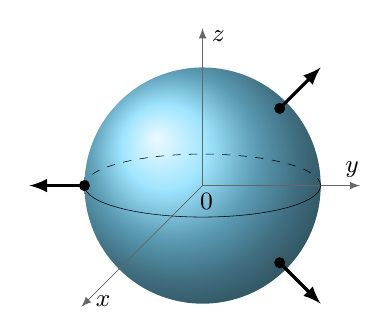
\begin{tikzpicture}
 \usetikzlibrary{arrows}
 \definecolor{spherecolor}{HTML}{80DCFF}
 \shade [ball color=spherecolor] (0,0) circle (1.5);
 \draw [black!60,line width=0.3pt,-latex] (0,0) -- (2,0,0);
 \draw [black!60,line width=0.3pt,-latex] (0,0) -- (0,2,0);
 \draw [black!60,line width=0.3pt,-latex] (0,0) -- (0,0,4);
 \pgfputat{\pgfpointxyz{1.9}{0.2}{0}}{\pgfbox[center,center]{\small $y$}};
 \pgfputat{\pgfpointxyz{0.2}{1.9}{0}}{\pgfbox[center,center]{\small $z$}};
 \pgfputat{\pgfpointxyz{0.2}{0}{3.8}}{\pgfbox[center,center]{\small $x$}};
 \pgfputat{\pgfpointxyz{0.05}{-0.2}{0}}{\pgfbox[center,center]{\small $0$}};
 \draw [line width=0.2pt] (-1.5,0) arc (180:360:1.5 and 0.4);
 \draw [dashed,line width=0.2pt] (1.5,0) arc (0:180:1.5 and 0.4);
 \fill (0.98,0.98) circle (2pt);
 \draw [line width=1.2pt,-latex] (0.98,0.98) -- (1.5,1.5);
 \fill (0.98,-0.98) circle (2pt);
 \draw [line width=1.2pt,-latex] (0.98,-0.98) -- (1.5,-1.5);
 \fill (-1.5,0) circle (2pt);
 \draw [line width=1.2pt,-latex] (-1.5,0) -- (-2.2,0);
\end{tikzpicture}
\end{figure}

Recall that normal vectors to a plane can point in two opposite directions. By an
\textbf{outward unit normal vector} to a surface $\superficie$, we will mean the unit vector that is normal to $\superficie$ and
points to the ``outer'' part of the surface.


  If $\superficie$ is some oriented surface with unit normal $\hat{ \vector{n}}$, then the amount of fluid flowing through $\superficie$ per unit time is exactly
  \begin{equation*}
    \diint_\superficie \vector{f} \bp \hat{ \vector{n}} \,  \d \S.
  \end{equation*}
  Note, both $\vector{f}$ and $\hat{ \vector{n}}$ above are \negrito{vector functions}, and $\vector{f} \bp \hat{ \vector{n}}: \superficie \to \bbR$ is a scalar function.
  The surface integral of this was defined in the previous section.




  \begin{exa}
    If $\superficie$ is the surface of a M\"obius strip, for instance, cannot be oriented.
  \end{exa}

  \begin{figure}[h!]
  \centering
  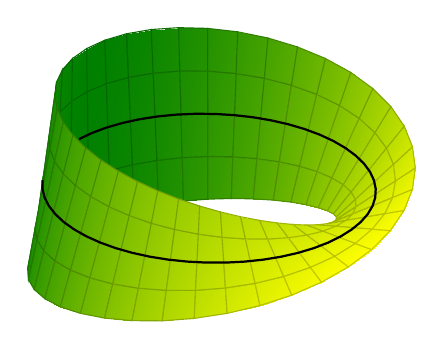
\begin{tikzpicture}
\begin{axis}[
    hide axis,
    view={40}{40}
]
\addplot3 [
    surf, shader=faceted interp,
    point meta=x,
    colormap/greenyellow,
    samples=40,
    samples y=5,
    z buffer=sort,
    domain=0:360,
    y domain=-0.5:0.5
] (
    {(1+0.5*y*cos(x/2)))*cos(x)},
    {(1+0.5*y*cos(x/2)))*sin(x)},
    {0.5*y*sin(x/2)});

\addplot3 [
    samples=50,
    domain=-145:180, % The domain needs to be adjusted manually, depending on the camera angle, unfortunately
    samples y=0,
    thick
] (
    {cos(x)},
    {sin(x)},
    {0});
\end{axis}
\end{tikzpicture}
\caption{The Moebius Strip is an example of a surface that is not orientable}
  \end{figure}










  \begin{definition}
    Let $(\superficie, \hat{ \vector{n}})$ be an oriented surface, and $\vector{f}:\superficie \to \bbR^3$ be a $C^1$ vector field.
    The \negrito{surface integral} of $\vector{f}$ over $\superficie$ is defined to be
    \begin{equation*}
      \diint_\superficie \vector{f} \bp \hat{ \vector{n}} \,  \d \S.
    \end{equation*}
  \end{definition}

  \begin{remark}
    Other common notation for the surface integral is
    \begin{equation*}
      \diint_\superficie \vector{f} \bp \hat{ \vector{n}} \,  \d \S
      = \diint_\superficie \vector{f} \bp  \d \vector{S}
     = \diint_\superficie \vector{f} \bp \d A
    \end{equation*}
  \end{remark}



  \vspace{3mm}
\begin{exa}\label{exmp:surfintex}
 Evaluate the surface integral $\diint\limits_{\superficie} \Dotprod{\vector{f}}{d{\superficie}}$, where
 $\vector{f}(x,y,z) = yz\vector{i} + xz\vector{j} + xy\vector{k}$ and $\superficie$ is the part of the plane $x+y+z=1$
 with $x \ge 0$, $y \ge 0$, and $z \ge 0$, with the outward unit normal $\vector{n}$ pointing in the positive $z$
 direction.

\end{exa}
\begin{figure}[h!]
\centering
 \begin{tikzpicture}
  \usetikzlibrary{arrows}
  \filldraw [black,fill=black!10] (1.5,0,0) -- (0,1.5,0) -- (0,0,1.5) -- (1.5,0,0);
  \draw [black!60,line width=0.3pt,-latex] (0,0) -- (2,0,0);
  \draw [black!60,line width=0.3pt,-latex] (0,0) -- (0,2,0);
  \draw [black!60,line width=0.3pt,-latex] (0,0) -- (0,0,2.5);
  \pgfputat{\pgfpointxyz{1.9}{0.2}{0}}{\pgfbox[center,center]{\small $y$}};
  \pgfputat{\pgfpointxyz{0.2}{1.9}{0}}{\pgfbox[center,center]{\small $z$}};
  \pgfputat{\pgfpointxyz{0.2}{0}{2.3}}{\pgfbox[center,center]{\small $x$}};
  \pgfputat{\pgfpointxyz{-0.1}{0.1}{0}}{\pgfbox[center,center]{\small $0$}};
  \node [below] at (1.5,0,0) {\small $1$};
  \node [left] at (0,1.5,0) {\small $1$};
  \node [left] at (0,0,1.4) {\small $1$};
  \node [left] at (0,0.8,0.5) {\small $\superficie$};
  \node [below] at (1.2,0,0.8) {\small $x+y+z=1$};
  \draw [dashed] (0,0,0.7) -- (0.7,0,0.7);
  \fill (0.48,0.48) circle (2pt);
  \draw [line width=1.2pt,-latex] (0.48,0.48) -- (1.1,1.1);
  \node [above right] at (1.02,1.02) {\small $\vector{n}$};
 \end{tikzpicture}
 \end{figure}

\begin{solu}

 Since the vector $\textbf{v} = (1,1,1)$ is normal to the plane $x+y+z=1$ (why?), then
 dividing \textbf{v} by its length yields the outward unit normal vector $\vector{n} = \left( \dfrac{1}{\sqrt{3}},
 \dfrac{1}{\sqrt{3}},\dfrac{1}{\sqrt{3}} \right)$. We now need to parametrize $\superficie$. As we can see from Figure
 projecting $\superficie$ onto the $xy$-plane yields a triangular region
 $R= \lbrace\,(x,y): 0 \le x \le 1,~ 0 \le y \le 1-x\,\rbrace$. Thus, using $(u,v)$ instead of $(x,y)$, we see that
 \begin{displaymath}
  x=u,~ y=v,~ z=1-(u+v),~~\text{for~} 0 \le u \le 1, 0 \le v \le 1-u
 \end{displaymath}
 is a parametrization of $\superficie$ over $\Omega$ (since $z=1-(x+y)$ on $\superficie$). So on $\superficie$,
 \begin{align*}
  \Dotprod{\vector{f}}{\vector{n}} ~&=~
   \Dotprod{(yz,xz,xy)}{\left( \dfrac{1}{\sqrt{3}},\dfrac{1}{\sqrt{3}},\dfrac{1}{\sqrt{3}} \right)}
   ~=~ \dfrac{1}{\sqrt{3}}(yz+xz+xy)\\[8pt]
   &=~ \dfrac{1}{\sqrt{3}}((x+y)z+xy)
   ~=~ \dfrac{1}{\sqrt{3}}((u+v)(1-(u+v))+uv)\\[8pt]
   &=~ \dfrac{1}{\sqrt{3}}((u+v)- (u+v)^2 + uv)
 \end{align*}
 for $(u,v)$ in $\Omega$, and for $\vector{r}(u,v)=x(u,v)\vector{i} + y(u,v)\vector{j} + z(u,v)\vector{k} = u\vector{i} +
 v\vector{j} + (1-(u+v))\vector{k}$ we have
 \begin{displaymath}
  \Crossprod{\dfrac{\partial \vector{r}}{\partial u}}{\dfrac{\partial \vector{r}}{\partial v}} ~=~
   \Crossprod{(1,0,-1)}{(0,1,-1)} ~=~ (1,1,1) \quad\Rightarrow\quad
  \Norm{\Crossprod{\dfrac{\partial \vector{r}}{\partial u}}{\dfrac{\partial \vector{r}}{\partial v}}} = \sqrt{3}~.
 \end{displaymath}
 Thus, integrating over $\Omega$ using vertical slices (e.g. as indicated by the dashed line in Figure 4.4.5) gives
 \begin{align*}
  \diint\limits_{\superficie} \Dotprod{\vector{f}}{\d \S} ~&=~
   \diint\limits_{\superficie} \Dotprod{\vector{f}}{\vector{n}}\,\d \S\\[6pt]
   &=~ \diint\limits_{\Omega} (\Dotprod{\vector{f}(x(u,v),y(u,v),z(u,v))}{\vector{n}})\,
   \Norm{\Crossprod{\dfrac{\partial \vector{r}}{\partial u}}{\dfrac{\partial \vector{r}}{\partial v}}}\,dv\,du\\[6pt]
   &=~ \dint_0^1 \dint_0^{1-u} \dfrac{1}{\sqrt{3}}((u+v)- (u+v)^2 + uv) \sqrt{3}\,dv\,du\\[8pt]
   &=~ \dint_0^1 \left( \dfrac{(u+v)^2}{2} - \dfrac{(u+v)^3}{3} + \dfrac{uv^2}{2}\,\Bigg|_{v=0}^{v=1-u} \right)\,du\\[8pt]
   &=~ \dint_0^1 \left( \dfrac{1}{6} + \dfrac{u}{2} - \dfrac{3u^2}{2} + \dfrac{5u^3}{6} \right)\,du\\[8pt]
   &=~ \dfrac{u}{6} + \dfrac{u^2}{4} - \dfrac{u^3}{2} + \dfrac{5u^4}{24}\,\Bigg|_0^1 ~=~ \dfrac{1}{8}~.
 \end{align*}

\end{solu}

  \begin{proposition}
    Let $\vector{r}:U \to \superficie$ be a parametrization of the oriented surface $(\superficie, \hat{ \vector{n}})$.
    Then either
    \begin{equation}\label{eqnSNorm}
      \hat{ \vector{n}} \circ \vector{r}
	= \dfrac{\partial_u\vector{r} \times \partial_v \vector{r}}{\abs{\partial_u\vector{r} \times \partial_v \vector{r}}}
    \end{equation}
    on all of $\superficie$, or
    \begin{equation}\label{eqnSNorm2}
      \hat{ \vector{n}} \circ \vector{r}
	= -\dfrac{\partial_u\vector{r} \times \partial_v \vector{r}}{\abs{\partial_u\vector{r} \times \partial_v \vector{r}}}
    \end{equation}
    on all of $\superficie$.
    Consequently, in the case~\eqref{eqnSNorm} holds, we have
    \begin{equation}\label{eqnSintDef}
      \diint_\superficie \vector{F} \bp \hat{ \vector{n}} \,  \d \S
	= \dint_U
	  (\vector{F} \circ \vector{r})  \bp (\partial_u\vector{r} \times \partial_v \vector{r}) \, \dA.
    \end{equation}
  \end{proposition}
  \begin{proof}
  The vector  $\partial_u\vector{r} \times \partial_v \vector{r}$ is \negrito{normal} to $\superficie$ and hence parallel to $\hat{ \vector{n}}$.
    Thus
    \begin{equation*}
      \hat{ \vector{n}} \bp \dfrac{\partial_u\vector{r} \times \partial_v \vector{r}}{\abs{\partial_u\vector{r} \times \partial_v \vector{r}}}
    \end{equation*}
    must be a function that only takes on the values $\pm 1$.
    Since $s$ is also continuous, it must either be identically $1$ or identically $-1$, finishing the proof.
  \end{proof}

  \begin{exa}
    Gauss's law sates that the total charge enclosed by a surface $\superficie$ is given by
    \begin{equation*}
      Q = \epsilon_0 \diint_\superficie  E \bp  \d \vector{S},
    \end{equation*}
    where $\epsilon_0$ the permittivity of free space, and $E$ is the electric field.
    By convention, the normal vector is chosen to be pointing outward.

    If $E(x) = e_3$, compute the charge enclosed by the top half of the hemisphere bounded by $\abs{x}  = 1$ and $x_3  = 0$.
  \end{exa}



  \section{Kelvin-Stokes Theorem}
  
  Given a surface $\superficie \subset{\mathbb R}^3$ with boundary $\partial \superficie$ you are free to chose the orientation of $\superficie$, i.e., the direction of the normal, but you have to orient $\superficie$ and $\partial \superficie$ coherently. This means that if you are an "observer" walking along the boundary of the surface with the normal as
your upright direction; you are moving in the positive direction if onto the surface the boundary  the interior of $\superficie$ is on \textit{to the left} of $\partial \superficie$.





  
  
\begin{exa}Consider the annulus
\[A:=\{(x,y,0)\ |\ a^2\leq x^2+y^2\leq b^2\}\]
in the $(x,y)$-plane, and from the two possible normal unit vectors $(0,0,\pm 1)$ choose $\hat{n}:=(0,0,1)$. If you are an "observer" walking along the boundary of the surface with the normal as $\hat{n}$ means  that the outer boundary circle  of $A$ should be oriented counterclockwise. Staring at the figure you can convince yourself that the inner boundary circle has to be oriented clockwise to make the interior of $A$ lie to the left of $\partial A$. One might write
$$\partial A=\partial D_b-\partial D_a\ ,$$
where $D_r$ is the disk of radius $r$ centered at the origin, and its boundary circle $\partial D_r$ is oriented counterclockwise.
\end{exa}


\begin{center}
 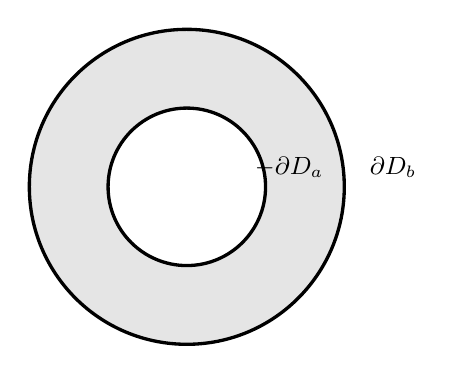
\begin{tikzpicture}
  \usetikzlibrary{arrows}
  \filldraw [black,line width=1.2pt,fill=black!10] (0,0) circle( 2);
  \filldraw [black,line width=1.2pt,fill=white] (0,0) circle (1);
  \node [above right] at (2.2,0) {\small $\partial D_b$};
  \node [above] at (1.3,0) {\small $-\partial D_a$};
%   \node at (0,1.35) {\small $\ssub{R}{1}$};
%   \node at (0,-1.35) {\small $\ssub{R}{2}$};
   \node [rotate=330] at (0.6964,0.69936) {\Large $\blacktriangleright$};
   \node [rotate=330] at (-0.6964,-0.69936) {\Large $\blacktriangleleft$};
   \node [rotate=-31] at (1.43,1.43) {\Large $\blacktriangleleft$};
   \node [rotate=-31] at (-1.43,-1.43) {\Large $\blacktriangleright$};
%   \draw [dashed] (2.5,0) -- (1.5,0);
%   \draw [dashed] (0.5,0) -- (-0.5,0);
%   \draw [dashed] (-1.5,0) -- (-2.5,0);
%   \draw [-latex] (1.8,0.15) -- (2.2,0.15);
%   \draw [latex-] (1.8,-0.15) -- (2.2,-0.15);
%   \draw [-latex] (-0.2,0.15) -- (0.2,0.15);
%   \draw [latex-] (-0.2,-0.15) -- (0.2,-0.15);
%   \draw [-latex] (-2.2,0.15) -- (-1.8,0.15);
%   \draw [latex-] (-2.2,-0.15) -- (-1.8,-0.15);
 \end{tikzpicture}
\end{center}


  \begin{theorem}[Kelvin–Stokes Theorem] \index{Kelvin–Stokes Theorem}
    Let $U \subseteq \bbR^3$ be a domain, $(\superficie, \hat{ \vector{n}}) \subseteq U$ be a bounded, oriented, piecewise $C^1$, surface whose boundary is the (piecewise $C^1$) curve $\caminho$.
    If $\funvect{f}:U \to \bbR^3$ is a $C^1$ vector field, then
    \begin{equation*}
      \dint_{\superficie} \curlb \funvect{f} \bp \hat{ \vector{n}} \,  \d \S
	= \doint_\caminho \funvect{f} \bp \d\ell.
    \end{equation*}
    Here $\caminho$ is traversed in the counter clockwise direction when viewed by an observer standing with his feet on the surface and head in the direction of the normal vector.
  \end{theorem}


  \begin{figure}[h!]
 \centering
 \begin{overpic}[width=7cm,tics=10]{./figs/TeoremaStokes.eps}
 % TeoremaStokes.eps: 0x0 pixel, 300dpi, 0.00x0.00 cm, bb=0 0 260 200
  \put (40,5) {$\caminho$}
  \put (61,65) {$\hat{ \vector{n}}$}
  \put (90,45) {$\superficie$}
    \put (27,64) {$\curlb \funvect{f}$}

  \end{overpic}
\end{figure}






  \begin{proof}
Let $\mathbf f= f_1\vector{i} + f_2\vector{j} + f_3\vector{k}$. Consider 
\[
  \nabla \times(f_1\vector{i}) = 
  \begin{vmatrix}
  \vector{i} & \vector{j} & \vector{k} \\
  \partial _x & \partial _y & \partial _z\\
  f_1 & 0 & 0 
\end{vmatrix}
= 
\vector{j} \frac{\partial f_1}{\partial z}
- \vector{k} \frac{\partial f_1}{\partial y}
\]
Then we have 
\begin{align*}
 \dint_\superficie[\nabla \times(f_1\vector{i})]\cdot \,\d S
  &=\dint_\superficie (\hat  n \cdot \nabla \times(f_1\vector{i})\,\d S\\
  &=\dint_\superficie \frac{\partial f_1}{\partial z}(\vector{j}\cdot \hat  n) - \frac{\partial f_1}{\partial y}(\vector{k} \cdot \hat  n)\,\d S
\end{align*}
We prove the theorem in the case  $\superficie$ is a graph of a function, i.e.,   $\superficie$ is parametrized as 
\[r=x \vector{i} +y \vector{j}+ g(x,y) \vector{k}\]
where $g(x,y): \Omega \to \bbR$. 
In this case the boundary $\caminho$ of $\superficie$ is given by the image of the curve $C$ boundary of $\Omega$:

	\begin{center}
\tdplotsetmaincoords{70}{120}
\pgfmathsetmacro{\rvec}{1.3}
\pgfmathsetmacro{\thetavec}{40}
\pgfmathsetmacro{\phivec}{60}

\begin{tikzpicture}[tdplot_main_coords,scale=.98]
\coordinate (O) at (0,0,0);
\draw[thick,-latex] (0,0,0) -- (3.5,0,0) node[anchor=north east]{$x$};
\draw[thick,-latex] (0,0,0) -- (0,3.5,0) node[anchor=north west]{$y$};
\draw[thick,-latex] (0,0,0) -- (0,0,2.2) node[anchor=south]{$z$};
\draw [fill = Blue!25] (2,2.15) circle (.82);
\draw[dashed] (2.3,1.38,0) -- (2.3,1.38,3);
\draw[dashed] (1.8,3,0.1) -- (1.8,3,2.7);
    \shade[ball color=Blue!20,opacity=0.2] (0,1.95,2)  arc (0:-180:.83cm and 5mm) arc (180:0:.83cm and .83cm);
\node at(2,3.6,3.5)  {$\superficie$};    
\node at (2,2.15,0) {$\Omega$};
\draw [->] (2,1.8,3.2) -- (2,1.2,3.7) node [above] {$\hat  n$};
    \draw (0,.1,1.6) arc (180:360:.78cm and 0.4cm);
    \draw[dashed] (0,0.1,1.7) arc (180:0:.78cm and 0.4cm); 
    \draw [->] (1,1.4,1.73) -- (1,1.41,1.73) node [below] {\small $\caminho$};
    \draw [->] (1,1.2,-.8) -- (1,1.21,-.8) node [below] {\small $C$};    
\end{tikzpicture}
\end{center}

Let the equation of $S$ be $z =g(x,y)$. Then we have
\[
  \hat  n =  \frac{-\partial g/\partial x \vector{i} - \partial g / \partial y \vector{j} + \vector{k}}{((\partial g/\partial x)^2 + (\partial g/\partial y)^2 + 1)^{1/2}}
\]
Therefore on $\Omega$:
\[
  \vector{j} \cdot \hat  n 
  = - \frac{\partial g}{\partial y}(\vector{k} \cdot \hat  n)
  = -\frac{\partial z}{\partial y}(\vector{k} \cdot \hat  n)
\]
Thus
\begin{align*}
  \dint_\superficie [\nabla \times(f_1\vector{i})]\cdot \d \S
  &= 
 \dint_\superficie \left(-\left.\frac{\partial f_1}{\partial y}\right|_{z,x} - \left.\frac{\partial f_1}{\partial z}\right|_{y,x}  \left.\frac{\partial z}{\partial y}\right|_{x}\right)(\vector{k}\cdot \hat  n)\,\d S\\
  \intertext{Using the chain rule for partial derivatives}
  &= -\dint_\superficie \left.\frac{\partial}{\partial y}\right|_{x}
  f_1(x,y,z)(\vector{k}\cdot \hat  n)\,\d S\\
  \intertext{Then:}
  &= -\dint_\Omega\frac{\partial}{\partial y}f_1(x,y,g)\,\d x\,\d y\\
  &= \oint_C f_1(x,y,f(x,y))
\end{align*}
with the last line following by using Green's theorem. However on $\caminho$ we have $z=g$ and 
\[
  \oint_C f_1(x,y,g)\,\d x = \oint_\caminho f_1(x,y,z)\,\d x
\]
We have therefore established that 
\[
 \dint_\superficie(\nabla \times\,f_1\vector{i})\cdot\,\d \vector{f} = 
  \oint_\caminho f_1\,\d x
\]
In a similar way we can show that 
\[
  \dint_\superficie(\nabla \times\,A_2\vector{j}) \cdot \d \vector{f} 
  = \oint_\caminho A_2\,\d y
\]
and 
\[
 \dint_\superficie(\nabla \times\,A_3\vector{k})\cdot \, \d \vector{f} = 
  \oint_\caminho A_3\,\d z
\]
and so the theorem is proved by adding all three results together. \end{proof}




  \begin{exa}\label{exa:stokesparab}
 Verify Stokes' Theorem for $\funvect{f}(x,y,z) = z\,\vector{i} + x\,\vector{j} + y\,\vector{k}$ when $\superficie$ is the
 paraboloid $z=x^2 + y^2$ such that $z \le 1$ .\vspace{2mm}
 \piccaption[]{\quad $z=x^2 + y^2$}\parpic[r]{\begin{tikzpicture}
  \usetikzlibrary{arrows}
  \definecolor{insideo}{HTML}{798084}
  \definecolor{insidei}{HTML}{F0F0F0}
  \definecolor{outer}{HTML}{424296}
  \definecolor{inner}{HTML}{D8D8FF}
  \shadedraw [left color=insideo,right color=insideo,middle color=insidei,line width=1.2pt] (0,3) ellipse (2 and 0.7);
  \shadedraw [left color=outer,right color=outer,middle color=inner]
  (2,3) arc (360:180:2 and 0.7) -- (-2,3) parabola bend (0,0) (2,3);
  \draw [dashed,line width=0.2pt] (-2,3) -- (2,3);
  \draw [dashed,line width=0.2pt] (-0.66,2.34) -- (0.66,3.66);
  \draw [line width=0.2pt] (-0.66,2.34) parabola [bend at end] (0,0);
  \draw [dashed,line width=0.2pt] (0.66,3.66) parabola [bend at end] (0,0);
  \draw [line width=0.2pt] (-1.25,1.2) arc (180:360:1.25 and 0.4);
  \draw [dashed,line width=0.2pt] (-1.25,1.2) arc (180:0:1.25 and 0.4);
  \draw [black!60,line width=0.3pt,-latex] (-2,0) -- (2,0,0);
  \draw [black!60,line width=0.3pt,-latex] (0,0) -- (0,4,0);
  \draw [black!60,line width=0.3pt,-latex] (0,0) -- (0,0,2);
  \draw [black,line width=1.1pt,-latex] (0,2.3) arc (270:325:2 and 0.7);
  \draw [black,line width=1.1pt,-latex] (0,3.7) arc (90:145:2 and 0.7);
  \draw [black,line width=1.2pt,-latex] (1,2.3938) -- (0.7,3.1);
  \pgfputat{\pgfpointxyz{1.9}{0.2}{0}}{\pgfbox[center,center]{\small $y$}};
  \pgfputat{\pgfpointxyz{0.2}{3.9}{0}}{\pgfbox[center,center]{\small $z$}};
  \pgfputat{\pgfpointxyz{0.2}{0}{1.8}}{\pgfbox[center,center]{\small $x$}};
  \pgfputat{\pgfpointxyz{0.05}{-0.2}{0}}{\pgfbox[center,center]{\small $0$}};
  \node [right] at (0.7,3.15) {\small $\vector{n}$};
  \node [right] at (1.5,3.7) {\small $C$};
  \node at (-1.3,0.7) {\small $\superficie$};
  \node [above left] at (0,3) {\small $1$};  
 \end{tikzpicture}\\
 \vspace{22mm}
 }

 \end{exa}
  \vspace{12mm}

\begin{solu} The positive unit normal vector to the surface\\$z=z(x,y)=x^2 + y^2$ is
 \begin{displaymath}
  \vector{n} ~=~
   \dfrac{-\dfrac{\partial z}{\partial x}\,\vector{i} - \dfrac{\partial z}{\partial y}\,\vector{j} +
   \vector{k}}{\sqrt{1 + \left( \dfrac{\partial z}{\partial x} \right)^2 +
   \left( \dfrac{\partial z}{\partial y} \right)^2}} ~=~
   \dfrac{-2x\,\vector{i} - 2y\,\vector{j} + \vector{k}}{\sqrt{1 + 4x^2 + 4y^2}} ~,
 \end{displaymath}
 and $\curlb~\vector{f}= (1-0)\,\vector{i}+(1-0)\,\vector{j}+(1-0)\,\vector{k} = \vector{i}+\vector{j}+\vector{k}$,
 so
 \begin{displaymath}
  \Dotprod{(\curlb~{\vector{f}}\,)}{\vector{n}} ~=~ (-2x-2y+1)/\sqrt{1 + 4x^2 + 4y^2} ~.
 \end{displaymath}

 \par\noindent
 Since $\superficie$ can be parametrized as $\vector{r}(x,y) = x\,\vector{i}+y\,\vector{j}+(x^2 + y^2 )\,\vector{k}$ for
 $(x,y)$ in the region $D = \lbrace \, (x,y):\,x^2 + y^2 \le 1 \,\rbrace$, then
 \begin{align*}
  \diint\limits_{\superficie} \Dotprod{(\curlb~{\vector{f}}\,)}{\vector{n}}\, \d \S ~&=~
   \diint\limits_{D} \Dotprod{(\curlb~{\vector{f}}\,)}{\vector{n}}\,
  \Norm{\Crossprod{\dfrac{\partial \vector{r}}{\partial x}}{\dfrac{\partial \vector{r}}{\partial y}}}\,dA\\
   &=~ \diint\limits_{D} \dfrac{-2x-2y+1}{\sqrt{1 + 4x^2 + 4y^2}}\,\sqrt{1 + 4x^2 + 4y^2}\,dA\\
   &=~ \diint\limits_{D} (-2x-2y+1)\,dA ~,~\text{so switching to polar coordinates gives}\\
   &=~ \dint_0^{2\pi} \dint_0^1 (-2r\cos \theta - 2r\sin \theta + 1)r\,dr\,d\theta\\
   &=~ \dint_0^{2\pi} \dint_0^1 (-2r^2 \cos \theta - 2r^2 \sin \theta + r)\,dr\,d\theta\\
   &=~ \dint_0^{2\pi} \left( -\dfrac{2r^3}{3} \cos \theta - \dfrac{2r^3}{3} \sin \theta +
   \dfrac{r^2}{2}\,\Big|_{r=0}^{r=1} \,\right)\,d\theta\\
   &=~ \dint_0^{2\pi} \left( -\dfrac{2}{3} \cos \theta - \dfrac{2}{3} \sin \theta + \dfrac{1}{2} \right)\,d\theta\\
   &=~ -\dfrac{2}{3} \sin \theta + \dfrac{2}{3} \cos \theta + \dfrac{1}{2}\theta\,\Big|_0^{2\pi} ~=~ \pi ~.
 \end{align*}

 \picskip{0}
 The boundary curve $C$ is the unit circle $x^2 + y^2 =1$ laying in the plane $z=1$ (see Figure), which can be
 parametrized as $x = \cos t$, $y = \sin t$, $z = 1$ for $0 \le t \le 2\pi$. So
 \begin{align*}
  \olineintvec{C}{f}{r} ~&=~ \dint_0^{2\pi} ((1)(-\sin t) + (\cos t)(\cos t) + (\sin t)(0))\,dt\\
   &=~ \dint_0^{2\pi} \left( -\sin t + \dfrac{1+\cos 2t}{2} \right) \,dt \quad \left( \text{here we used $\cos^2 t =
   \dfrac{1+\cos 2t}{2}$} \right)\\
   &=~ \cos t + \dfrac{t}{2} + \dfrac{\sin 2t}{4}\,\Big|_0^{2\pi} ~=~ \pi ~.
 \end{align*}
 So we see that $\olineintvec{C}{f}{r}=\diint\limits_{\superficie} \Dotprod{(\curlb~{\vector{f}}\,)}{\vector{n}}
 \, \d \S$, as predicted by Stokes' Theorem.
\end{solu}

The line integral in the preceding example was far simpler to calculate than the surface integral, but this will not
always be the case.


\begin{exa}
  Let $S$ be the section of a sphere of radius $a$ with $0 \leq \theta \leq \alpha$. In spherical coordinates,
  \[
    \d \S = a^2 \sin \theta \vector{e}_r \;\d \theta\;\d \varphi.
  \]
  Let $\vector{F} = (0, xz, 0)$. Then $\nabla \times \vector{F} = (-x, 0, z)$. Then
  \[
    \dint_S \nabla\times \vector{F}\bp \d \vector{S} = \pi a^3 \cos\alpha\sin^2 \alpha.
  \]
  Our boundary $\partial C$ is
  \[
    \vector{r}(\varphi) = a(\sin \alpha\cos \varphi, \sin \alpha\sin \varphi, \cos \alpha).
  \]
  The right hand side of Stokes' is
  \begin{align*}
    \dint_C \vector{F}\bp \d \ell &= \dint_0^{2\pi}\underbrace{a\sin \alpha\cos \varphi}_{x}\underbrace{\vphantom{\varphi}a\cos\alpha}_z \underbrace{a\sin \alpha\cos\varphi\;\d \varphi}_{\d y}\\
    &= a^3\sin^2\alpha\cos\alpha\dint_0^{2\pi}\cos^2\varphi\;\d \varphi\\
    &= \pi a^3\sin^2\alpha\cos\alpha.
  \end{align*}
  So they agree.
\end{exa}


  \begin{remark}
    The rule determining the direction of traversal of $\caminho$ is often called the \negrito{right hand rule}.
    Namely, if you put your right hand on the surface with thumb aligned with $\hat{ \vector{n}}$, then $\caminho$ is traversed in the pointed to by your index finger.
  \end{remark}

  \begin{remark}
    If the surface $\superficie$ has holes in it, then (as we did with Greens theorem) we orient each of the holes clockwise, and the exterior boundary counter clockwise following the right hand rule.
    Now Kelvin–Stokes theorem becomes
    \begin{equation*}
      \dint_{\superficie} \curlb \funvect{f} \bp \hat{ \vector{n}} \,  \d \S
	= \dint_{\partial \superficie} \funvect{f} \bp \d\ell,
    \end{equation*}
    where the line integral over $\partial \superficie$ is defined to be the sum of the line integrals over each component of the boundary.
  \end{remark}

  \begin{remark}
    If $\superficie$ is contained in the $x, y$ plane and is oriented by choosing $\hat{ \vector{n}} = e_3$, then Kelvin–Stokes theorem reduces to Greens theorem.
  \end{remark}

  Kelvin–Stokes theorem allows us to quickly see how the curl of a vector field measures the infinitesimal circulation.
  \begin{proposition}
    Suppose a small, rigid paddle wheel of radius $a$ is placed in a fluid with center at $x_0$ and rotation axis parallel to $\hat{ \vector{n}}$.
    Let $v:\bbR^3 \to \bbR^3$ be the vector field describing the velocity of the ambient fluid.
    If $\omega$ the angular speed of rotation of the paddle wheel about the axis $\hat{ \vector{n}}$, then
    \begin{equation*}
      \lim_{a \to 0} \omega = \dfrac{\curlb v(x_0) \bp \hat{ \vector{n}}}{2}.
    \end{equation*}
  \end{proposition}
  \begin{proof}
    Let $\superficie$ be the surface of a disk with center $x_0$, radius $a$, and face perpendicular to $\hat{ \vector{n}}$, and $\caminho = \partial \superficie$.
    (Here $\superficie$ represents the face of the paddle wheel, and $\caminho$ the boundary.)
    The angular speed $\omega$ will be such that
    \begin{equation*}
      \doint_\caminho (v - a \omega \hat \tau) \bp \d\ell = 0,
    \end{equation*}
    where $\hat \tau$ is a unit vector tangent to $\caminho$, pointing in the direction of traversal.
    Consequently
    \begin{equation*}
      \omega
	= \dfrac{1}{2 \pi a^2} \doint_\caminho v \bp \d\ell
	= \dfrac{1}{2 \pi a^2} \diint_\superficie \curlb v \bp \hat{ \vector{n}} \,  \d \S
	\xrightarrow{a \to 0} \dfrac{\curlb v(x_0) \bp \hat{ \vector{n}}}{2}.
	\qed
    \end{equation*}
  \end{proof}

%   \begin{remark}
%     If the axis of the paddle wheel is chosen to maximise the angular velocity, we see that $\hat{ \vector{n}}$ must be parallel to $\curlb v$, and the maximum angular velocity is exactly $\abs{\curlb v} / 2$.
%     Treating a small sphere as a combination of paddle wheels will prove the rotation formula claimed in Remark~\ref{rmkBallRotating}.
%   \end{remark}


\begin{exa}
 Let $\superficie$ be the elliptic paraboloid $z=\dfrac{x^2}{4}+\dfrac{y^2}{9}$ for $z \le 1$, and let $C$ be its boundary
 curve.
 Calculate $\olineintvec{C}{f}{r}$ for $\funvect{f}(x,y,z)=(9xz+2y)\vector{i}+(2x+y^2 )\vector{j}+(-2y^2 +2z)\vector{k}$,
 where $C$ is traversed counterclockwise.\vspace{1mm}
\end{exa}
\begin{solu}
 The surface is similar to the one in Example \ref{exa:stokesparab}, except now the
 boundary curve $C$ is the ellipse $\dfrac{x^2}{4}+\dfrac{y^2}{9}=1$ laying in the plane $z=1$. In this case, using
 Stokes' Theorem is easier than computing the line integral directly. As in Example \ref{exa:stokesparab}, at each
 point $(x,y,z(x,y))$ on the surface $z=z(x,y)=\dfrac{x^2}{4}+\dfrac{y^2}{9}$ the vector
 \begin{displaymath}
  \vector{n} ~=~
   \dfrac{-\dfrac{\partial z}{\partial x}\,\vector{i} - \dfrac{\partial z}{\partial y}\,\vector{j} +
   \vector{k}}{\sqrt{1 + \left( \dfrac{\partial z}{\partial x} \right)^2 +
   \left( \dfrac{\partial z}{\partial y} \right)^2}} ~=~
   \dfrac{-\dfrac{x}{2}\,\vector{i} - \dfrac{2y}{9}\,\vector{j} + \vector{k}}{\sqrt{1 +\dfrac{x^2}{4}+
    \dfrac{4y^2}{9}}} ~,
 \end{displaymath}
 is a positive unit normal vector to $\superficie$. And calculating the curl of $\vector{f}$ gives
 \begin{displaymath}
  \curlb~\vector{f} ~=~ (-4y-0)\vector{i} ~+~ (9x-0)\vector{j} ~+~ (2-2)\vector{k} ~=~ -4y\,\vector{i} ~+~ 9x\,\vector{j} ~+~
   0\,\vector{k}~,
 \end{displaymath}
 so
 \begin{displaymath}
  \Dotprod{(\curlb~{\vector{f}}\,)}{\vector{n}} ~=~ \dfrac{(-4y)(-\dfrac{x}{2})+(9x)(-\dfrac{2y}{9})+
   (0)(1)}{\sqrt{1 +\dfrac{x^2}{4}+\dfrac{4y^2}{9}}} ~=~ \dfrac{2xy-2xy+0}{\sqrt{1 +\dfrac{x^2}{4}+\dfrac{4y^2}{9}}} ~=~ 0~,
 \end{displaymath}
 and so by Stokes' Theorem
 \begin{displaymath}
  \olineintvec{C}{f}{r} ~=~ \diint\limits_{\superficie} \Dotprod{(\curlb~{\vector{f}}\,)}{\vector{n}}\, \d \S ~=~
   \diint\limits_{\superficie} 0\, \d \S ~=~ 0 ~.
 \end{displaymath}
\end{solu}



  \section{Divergence Theorem}


  \begin{theorem}[Divergence Theorem]
    Let $U \subseteq \bbR^3$ be a bounded domain whose boundary is a (piecewise) $C^1$ surface denoted by $\partial U$.
    If $\vector{f}:U \to \bbR^3$ is a $C^1$ vector field, then
    \begin{equation*}
      \diiint_U (\grad \bp \vector{f}) \, \d V = \doiint_{\partial U} \vector{f} \bp \hat{ \vector{n}} \,  \d \S,
    \end{equation*}
    where $\hat{ \vector{n}}$ is the outward pointing unit normal vector.
  \end{theorem}

  \begin{remark}
    Similar to our convention with line integrals, we denote surface integrals over \negrito{closed surfaces} with the symbol $\doiint$.
  \end{remark}

  \begin{remark}
    Let $B_R = B(x_0, R)$ and observe
    \begin{equation*}
      \lim_{R \to 0} \dfrac{1}{\vol{\partial B_R}} \dint_{\partial B_R} \vector{f} \bp \hat{ \vector{n}} \,  \d \S
      = \lim_{R \to 0} \dfrac{1}{\vol{\partial B_R}} \dint_{B_R} \grad \bp \vector{f} \, \d V = \grad \bp \vector{f}(x_0),
    \end{equation*}
    which justifies our intuition that $\grad \bp \vector{f}$ measures the outward flux of a vector field.
  \end{remark}

  \begin{remark}
    If $V \subseteq \bbR^2$, $U = V \times [a, b]$ is a cylinder, and $\vector{f}:\bbR^3 \to R^3$ is a vector field that doesn't depend on $x_3$, then the divergence theorem reduces to Greens theorem.
  \end{remark}

  \begin{proof}[Proof of the Divergence Theorem]
    Suppose first that the domain $U$ is the unit cube $(0, 1)^3 \subseteq \bbR^3$.
    In this case
    \begin{equation*}
      \diiint_U \grad \bp \vector{f} \, \d V
	= \diiint_U (\partial_1 v_1 + \partial_2 v_2 + \partial_3 v_3) \, \d V.
    \end{equation*}
    Taking the first term on the right, the fundamental theorem of calculus gives
    \begin{align*}
      \diiint_U \partial_1 v_1 \, \d V
	&= \dint_{x_3 = 0}^1 \dint_{x_2 = 0}^1 ( v_1(1, x_2, x_3) - v_1( 0, x_2, x_3) ) \, \dx_2 \, \dx_3
	\\
	&= \dint_L v \bp \hat{ \vector{n}} \,   \d \S+ \dint_R v \bp \hat{ \vector{n}} \,  \d \S,
    \end{align*}
    where $L$ and $B$ are the left and right faces of the cube respectively.
    The $\partial_2 v_2$ and $\partial_3 v_3$ terms give the surface integrals over the other four faces.
    This proves the divergence theorem in the case that the domain is the unit cube.

%     Now given an arbitrary domain $U$, suppose there exists a $C^2$ coordinate change function $\varphi: C \to U$.
%     By interchanging $x_1$ and $x_2$ if necessary, we can guarantee $\det(\D\varphi) > 0$ in all of $U$.
%     Using the coordinate change formula for surface integrals  observe
%     \begin{equation*}
%       \dint_{\partial U} \vector{f} \bp \hat{ \vector{n}} \,  \d \S
% 	= \\dint_{\partial U}
% 	    \left[ (\D\varphi)^T \vector{f} \circ \varphi \right] \bp \hat{ \vector{n}} \,  \d \S
% 	= \diiint_U \grad \bp w \, \d V,
%     \end{equation*}
%     where
%     \begin{equation*}
%       \vector{w} = (\D\varphi)^T \, \vector{f} \circ \varphi.
%     \end{equation*}
%     Now, with the product and chain rule, we compute
%     \begin{equation*}
%       \grad \bp \vector{w} = \det(\D\varphi) \, (\grad \bp \vector{f}) \circ \varphi,
%     \end{equation*}
%     and by the coordinate change for volume integrals
%     \begin{equation*}
%       \dint_{\partial U} \vector{v} \bp \hat{ \vector{n}} \,  \d \S
%       = \diiint_U \grad \bp \vector{w} \, \d V
%       = \dint_U \grad \bp \vector{f} \, \d V,
%     \end{equation*}
%     concluding the proof.
  \end{proof}


  \begin{exa}
 Evaluate $\diint\limits_{\superficie} \Dotprod{\vector{f}}{\d \S}$, where $\funvect{f}(x,y,z) = x\vector{i} +
  y\vector{j} + z\vector{k}$ and $\superficie$ is the unit sphere $x^2 + y^2 + z^2 = 1$.\vspace{1mm}
\end{exa}
\begin{solu}We see that $\text{div}~\vector{f} = 1+1+1=3$, so
 \begin{align*}
  \diint\limits_{\superficie} \Dotprod{\vector{f}}{\d \S} ~&=~
  \iiint\limits_{S} \text{div}~\vector{f} ~\d V
  ~=~ \iiint\limits_{S} 3 ~\d V\\
  &=~ 3 \iiint\limits_{S} 1 ~\d V
  ~=~ 3\,\text{vol}(S) ~=~ 3\cdot \dfrac{4\pi (1)^3}{3} ~=~ 4\pi ~.
 \end{align*}
\end{solu}


\begin{exa}
  Consider a hemisphere.
  \begin{center}
    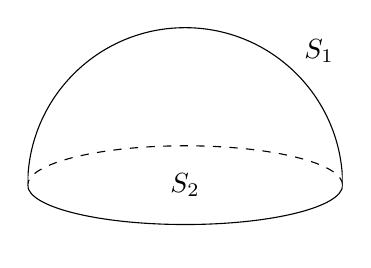
\begin{tikzpicture}
      \begin{scope}
        \clip (-2, 2) rectangle (2, 0);
        \draw circle [radius=2];
        \draw [dashed] circle [x radius = 2, y radius = 0.5];
      \end{scope}
      \begin{scope}
        \clip (-2, 0) rectangle (2, -0.7);
        \draw circle [x radius = 2, y radius = 0.5];
      \end{scope}
      \node {$S_2$};
      \node at (1.7, 1.7) {$S_1$};
    \end{tikzpicture}
  \end{center}

  $V$ is a solid hemisphere
  \[
    x^2 + y^2 + z^2 \leq a^2, \quad z \geq 0,
  \]
  and $\partial V = S_1 + S_2$, the hemisphere and the disc at the bottom.

  Take $\vector{F} = (0, 0, z + a)$ and $\nabla \bp \vector{F} = 1$. Then
  \[
    \dint_V\nabla \bp \vector{F}\;\d V = \dfrac{2}{3}\pi a^3,
  \]
  the volume of the hemisphere.

  On $S_1$,
  \[
    \d \S = \vector{n}\; \d \S= \dfrac{1}{a}(x, y, z)\;\d \S.
  \]
  Then
  \[
    \vector{F}\bp \d \vector{S} = \dfrac{1}{a}z(z + a)\; \d \S= \cos \theta a(\cos \theta + 1)\underbrace{a^2\sin \theta\;\d \theta\;\d \varphi}_{\d \S}.
  \]
  Then
  \begin{align*}
    \dint_{S_1}\vector{F}\bp \d \vector{S} &= a^3\dint_0^{2\pi}\d \varphi \dint_0^{\pi/2}\sin \theta(\cos^2\theta + \cos \theta)\;\d \theta\\
    &= 2\pi a^3 \left[\dfrac{-1}{3}\cos^3 \theta - \dfrac{1}{2}\cos^2 \theta\right]_0^{\pi/2}\\
    &= \dfrac{5}{3}\pi a^3.
  \end{align*}
  On $S_2$, $\d \S = \vector{n}\; \d \S= -(0, 0, 1)\;\d \S$. Then $\vector{F}\bp \d \vector{S} = -a\;\d \S$. So
  \[
    \dint_{S_2} \vector{F}\bp \d \vector{S} = -\pi a^3.
  \]
  So
  \[
    \dint_{S_1}\vector{F}\bp \d \vector{S} +\dint_{S_2}\vector{F}\bp \d \vector{S} = \left(\dfrac{5}{3} - 1\right)\pi a^3 = \dfrac{2}{3}\pi a^3,
  \]
  in accordance with Gauss' theorem.
\end{exa}








%
% \subsection{Sorces and Sinks}
% \todoin{write}

\subsection{Gauss's Law For  Inverse-Square  Fields}

  \begin{proposition}[Gauss's gravitational law]
    Let $g:\bbR^3 \to \bbR^3$ be the gravitational field of a mass distribution (i.e. $g(x)$ is the force experienced by a point mass located at $x$).
    If $\superficie$ is any closed $C^1$ surface, then
    \begin{equation*}
      \doint_\superficie g \bp \hat{ \vector{n}} \,   \d \S= - 4 \pi G M,
    \end{equation*}
    where $M$ is the mass enclosed by the region $\superficie$.
    Here $G$ is the gravitational constant, and $\hat{ \vector{n}}$ is the outward pointing unit normal vector.
  \end{proposition}

  \begin{proof}
    The core of the proof is the following calculation.
    Given a fixed $y \in \bbR^3$, define the vector field $\funvect{f}$ by
    \begin{equation*}
      \funvect{f}(x) = \dfrac{\vector{x}-\vector{y}}{\norm{\vector{x} - \vector{y}}^3}.
    \end{equation*}
    The vector field $-Gm \funvect{f}(x)$ represents the gravitational field of a mass located at $\vector{y}$
    Then
    \begin{equation}\label{eqnGauss1}
      \doint_\superficie  \funvect{f} \bp \hat{ \vector{n}} \,   \d \S=
      \begin{cases*}
	4\pi & if $\vector{y}$ is in the region enclosed by $\superficie$,\\
	0 & otherwise.
      \end{cases*}
    \end{equation}
    For simplicity, we subsequently assume $\vector{y} = \vector{0}$.

    To prove~\eqref{eqnGauss1}, observe
    \begin{equation*}
      \grad \bp \funvect{f} = 0,
    \end{equation*}
    when $\vector{x} \neq \vector{0}$.
    Let $U$ be the region enclosed by $\superficie$.
    If $\vector{0} \not\in U$, then the divergence theorem will apply to in the region $U$ and we have
    \begin{equation*}
      \doint_\superficie g \bp \hat{ \vector{n}} \,   \d \S= \dint_U \grad \bp g \, \d V = 0.
    \end{equation*}

    On the other hand, if $\vector{0} \in U$, the divergence theorem will not directly apply, since $\funvect{f} \not \in C^1(U)$.
    To circumvent this, let $\epsilon > 0$ and $U' = U - B(0, \epsilon)$, and $\superficie'$ be the boundary of $U'$.
    Since $0 \not \in U'$, $\funvect{f}$ is $C^1$ on all of $U'$ and the divergence theorem  gives
    \begin{equation*}
      0 = \dint_{U'} \grad \bp \funvect{f} \, \d V = \dint_{\partial U'} \funvect{f} \bp \hat{ \vector{n}} \,  \d \S,
    \end{equation*}
    and hence
    \begin{equation*}
      \doint_{\superficie} \funvect{f} \bp \hat{ \vector{n}} \,  \d \S
	= -\doint_{\partial B(0, \epsilon)} \funvect{f} \bp \hat{ \vector{n}} \,  \d \S
	= \doint_{\partial B(0, \epsilon)} \dfrac{1}{\epsilon^2} \,  \d \S
	= -4\pi,
    \end{equation*}
    as claimed.
    (Above the normal vector on $\partial B(0, \epsilon)$ points outward with respect to the domain $U'$, and \emph{inward} with respect to the ball $B(0, \epsilon)$.)

    Now, in the general case, suppose the mass distribution has density $\rho$.
    Then  the gravitational field $g(x)$ will be the super-position of the gravitational fields at $x$ due to a point mass of size $\rho(y) \, \d V$ placed at $y$.
    Namely, this means
    \begin{equation*}
      g(x) = -G \dint_{\bbR^3} \dfrac{\rho(y) (x - y)}{\abs{x - y}^3} \, \d V(y).
    \end{equation*}
    Now using Fubini's theorem,
    \begin{multline*}
      \diint_\superficie g(x) \bp \hat{ \vector{n}}(x) \,  \d \S(x)
	= -G \dint_{y \in \bbR^3} \rho(y) \dint_{x \in \superficie} \dfrac{x -y}{\abs{x - y}^3} \bp \hat{ \vector{n}}(x) \,  \d \S(x) \, \d V(y)
	\\
	= -4 \pi G \dint_{y \in U} \rho(y) \, \d V(y) = -4 \pi GM,
    \end{multline*}
    where the second last equality followed from~\eqref{eqnGauss1}.
  \end{proof}
    
    
    

\begin{exa}
 A system of electric charges has a \emph{charge density} $\rho (x,y,z)$ and produces an electrostatic field
 $\vector{E}(x,y,z)$ at points $(x,y,z)$ in space. \emph{Gauss' Law} states that
 \begin{displaymath}
  \diint\limits_{\superficie} \Dotprod{\vector{E}}{\d \S} ~=~ 4\pi\,\iiint\limits_{S} \rho ~\d V
 \end{displaymath}
 for any closed surface $\superficie$ which encloses the charges, with $S$ being the solid region enclosed by $\superficie$.
 Show that $\Dotprod{\nabla}{\vector{E}} = 4\pi\rho$. This is one of \emph{Maxwell's Equations}.\footnote{In Gaussian
 (or CGS) units.}\vspace{1mm}
\end{exa}
\begin{solu}
 By the Divergence Theorem, we have
 \begin{align*}
  \iiint\limits_{S} \Dotprod{\nabla}{\vector{E}} ~\d V ~&=~ \diint\limits_{\superficie} \Dotprod{\vector{E}}{\d \S}\\
   &=~ 4\pi\,\iiint\limits_{S} \rho ~\d V \quad\text{by Gauss' Law, so combining the integrals gives}\\
   \iiint\limits_{S} ( \Dotprod{\nabla}{\vector{E}} - 4\pi\rho ) ~\d V ~&=~ 0 \quad\text{, so}\\
   \Dotprod{\nabla}{\vector{E}} - 4\pi\rho ~&=~ 0 \quad\text{since $\superficie$ and hence $S$ was arbitrary, so}\\
   \Dotprod{\nabla}{\vector{E}} ~&=~ 4\pi\rho ~.
 \end{align*}
\end{solu}





%   \section{Change of Variable in Surface Integration}
% Suppose we have a surface $S$ which is parameterized by the quantities $u_1,\, u_2$. We can therefore write that on $S$:
% \[
%   x = x(u_1,u_2),\; y= y(u_1,u_2),\; z = z(u_1,u_2)
% \]
% [For example, if $S$ is the surface of a sphere of unit radius, we have $x = \sin\theta\cos\phi,\, y = \sin\theta\sin\phi,\, z = \cos\theta$
% and so we can take $u_1 = \theta,\, u_2 = \phi$.]
%
% We can consider the surface to be comprised of arbitrarily small parallelograms whose sides are
% obtained by keeping either $u_2$ or $u_2$ constant:
% %  \begin{center}
% %  \includegraphics[width=3cm]{fig24.jpg}
% %  \end{center}
%
% i.e.
% \begin{align*}\\[-1cm]
%    \d \S
%   &= \text{ Area of parallelogram with sides } \dfrac{\partial \vector r}{\partial u_1}\d u_1 \text{ and } \dfrac{\partial \vector r}{\partial u_2}\d u_2\\
%   &= |\vector J|\,\d u_1\d u_2
% \end{align*}
% %where
%
% \begin{definition}[Jacobian]
% The \negrito{Jacobian}, $\vector J$, is given by
% \[
%   \vector J = \dfrac{\partial \vector r}{\partial u_1} \times \dfrac{\partial \vector r}{\partial u_2}
% \]
% \end{definition}
%
% This result is particularly useful when using a substitution in a surface integral, as we can write
% \[
%   \d\dint_\superficie f(x,y,z)\, \d \S= \d\dint_\superficie F(u_1,u_2)|\vector J|\,\d u_1\d u_2
% \]
% where $F(u_1,u_2) = f(x(u_1,u_2),y(u_1,u_2),z(u_1,u_2))$.
%
% If $S$ is a region $\Omega$ in the $x-y$ plane (i.e. $z=0$ on $\Omega$), the result reduces to
% \[
%   \dint_R f(x,y)\,\d x\d y
%   = \dint_R F(u_1,u_2)|J|\,\d u_1\d u_2
% \]
% where $J$ is now a scalar given by
% \[
%   J =
%   \begin{vmatrix}
%   \partial x/\partial u_1 & \partial y/\partial u_1\\
%   \partial x/\partial u_2 & \partial y/\partial u_2
%   \end{vmatrix}
% \]
% Note that since $\d x\,\d y = |J|\d u_1\d u_2$,
% it follows that $\d u_1\d u_2 = (1/|J|)\,\d x\d y$, and hence
% \[
%   |1/J| =
%   \left|\begin{vmatrix}
%   	\partial u_1/\partial x & \partial u_2/\partial x\\
%   	\partial u_1/\partial y & \partial u_2/\partial y
%   \end{vmatrix}\right|
% \]
% which is a useful result. These formulae apply for both orthogonal and non-orthogonal transformations.\\
%
%
% \begin{exa}
% Evaluate the integral $\d\dint_\superficie \sqrt{1 + x^2 + y^2}\,\d \S$, where $S$ is the surface of the helicoid (see picture below):
% \[
%   x = u\cos v,\; y = u\sin v,; z =v
% \]
% with $0 \leq u \leq 4$ and $0 \leq v \leq 4\pi$.
% % \begin{center}
% % \includegraphics[width=5cm]{fig25.jpg}
% % \end{center}
%
%
% We need to find
% \begin{align*}
% \vector J &= \dfrac{\partial \vector r}{\partial u} \times \dfrac{\partial \vector r}{\partial v}\\[.2cm]
% &= \begin{vmatrix}
%  \hat i & \hat j & \hat k\\
%  \partial x/\partial u & \partial y/\partial u & \partial z/\partial u\\
%  \partial x /\partial v	&\partial y/\partial v & \partial z/\partial v\\
%  \end{vmatrix}\\[.2cm]
%  &=
%  \begin{vmatrix}
%  	 \hat i & \hat j & \hat k\\
% \cos v & \sin v & 0\\
% -u\sin v & u\cos v & 1
%  \end{vmatrix}\\[.2cm]
% &= (\sin v)\hat i - (\cos v)\hat j + \underbrace{(u\cos^2v + u\sin^2v)}_u\hat k\\
% \end{align*}
% Therefore
% \[
%   |\vector J| = \sqrt{\sin^2v + \cos^2v + u^2} = \sqrt{1+u^2}
% \]
%
% Also
% \begin{align*}
%   \sqrt{1+x^2+y^2} = \sqrt{1 + u^2\cos^2v + u^2\sin^2v} = \sqrt{1+u^2}
% \end{align*}
% \begin{align*}
%   \implies \d\dint_\superficie \sqrt{1 + x^2 + y^2}\, \d \S
%   &= \dint_S \sqrt{1+ u^2}|\vector J|\,\d u\d v\\
%   &= \dint_{v=0}^{4\pi} \dint_{u=0}^4 (1+u^2)\,\d u \d v\\
%   &= 4\pi \left[u + \dfrac{u^3}{3}\right]_0^4\\
%   &= 4\pi \left(4 + \dfrac{64}{3}\right)\\
%   &= \dfrac{304\pi}{3}
% \end{align*}
% \end{exa}
%
% \vspace*{.5cm}
%
% % \begin{center}
% % \includegraphics[width=6cm]{mom.pdf}
% % \end{center}

\section{Applications of Surface Integrals}
\subsection{Conservative and Potential Forces } \label{conservative-potencial}






  We've seen before that any potential force must be conservative.
  We demonstrate  the converse here.

  \begin{theorem}\label{thmPotentialForce}
    Let $U \subseteq \bbR^3$ be a simply connected domain, and $\funvect{f}:U \to \bbR^3$ be a $C^1$ vector field.
    Then $\funvect{f}$ is a conservative force, if and only if $\funvect{f}$ is a potential force, if and only if $\curlb \funvect{f} = 0$.
  \end{theorem}


  \begin{proof}
    Clearly, if $\funvect{f}$ is a potential force, equality of mixed partials shows $\curlb \funvect{f} = 0$.
    Suppose now $\curlb \funvect{f} = 0$.
    By Kelvin–Stokes theorem
    \begin{equation*}
      \doint_\caminho \funvect{f} \bp \d\ell = \dint_{\superficie} \curlb \funvect{f} \bp \hat{ \vector{n}} \,   \d \S= 0,
    \end{equation*}
    and so $\funvect{f}$ is conservative.
    Thus to finish the proof of the theorem, we only need to show that a conservative force is a potential force.
    We do this next.

    Suppose $\funvect{f}$ is a conservative force.
    Fix $x_0 \in U$ and define
    \begin{equation*}
      V(x) = -\dint_\caminho \funvect{f} \bp \d\ell,
    \end{equation*}
    where $\caminho$ is \emph{any} path joining $x_0$ and $x$ that is completely contained in $U$.
    Since $\funvect{f}$ is conservative, we seen before that the line integral above \emph{will not} depend on the path itself but only on the endpoints.

    Now let $h > 0$, and let $\caminho$ be a path that joins $x_0$ to $a$, and is a straight line between $a$ and $a + h e_1$.
    Then
    \begin{equation*}
      -\partial_1 V(a) = \lim_{h \to 0} \dfrac{1}{h} \dint_{a_1}^{a_1 + h} F_1( a + t e_1) \, \dt= F_1(a).
    \end{equation*}
    The other partials can be computed similarly to obtain $\funvect{f} = -\grad V$ concluding the proof.
  \end{proof}

%   \begin{remark}
%     Let $U = \bbR^3 - \set{ te_3 \st t \in \bbR }$, and define $\funvect{f}: U \to \bbR^3$ by
%     \begin{equation*}
%       \funvect{f}(x) = \dfrac{1}{x_1^2 + x_2^2} \colvec{ -x_2\\x_1\\0}.
%     \end{equation*}
%     It's easy to check that $\funvect{f} \in C^1(U)$ and $\curlb \funvect{f} = 0$.
%     However, we claim there does not exist any $V:U \to \bbR$ such that $\funvect{f} = -\grad V$.
%     To see this let $\caminho$ be the unit circle with center $0$ contained in the $x_1$-$x_2$ plane.
%     A calculation we've done before shows
%     \begin{equation*}
%       \doint_\caminho \funvect{f} \bp \d\ell = 2\pi \neq 0.
%     \end{equation*}
%     But by the fundamental theorem we know $\doint \grad V \bp \d\ell = 0$ for any closed curve, and thus $\funvect{f}$ cannot equal $-\grad V$ for any $V \in C^1(U)$.
%   \end{remark}


\subsection{Conservation laws}
\begin{df}[Conservation equation]
  Suppose we are interested in a quantity $Q$. Let $\rho(\vector{r}, t)$ be the amount of stuff per unit volume and $\vector{j}(\vector{r}, t)$ be the flow rate of the quantity (eg if $Q$ is charge, $j$ is the current density).

  The conservation equation is
  \[
    \dfrac{\partial \rho}{\partial t} + \nabla\bp \vector{j} = 0.
  \]
\end{df}
This is stronger than the claim that the total amount of $Q$ in the universe is fixed. It says that $Q$ cannot just disappear here and appear elsewhere. It must continuously flow out.

In particular, let $V$ be a fixed time-independent volume with boundary $S = \partial V$. Then
\[
  Q(t) = \dint_V \rho (\vector{r}, t)\; \d V
\]
Then the rate of change of amount of $Q$ in $V$ is
\[
  \dfrac{\d Q}{\d t} = \dint_V \dfrac{\partial \rho }{\partial t}\;\d V = -\dint_V \nabla \bp \vector{j}\;\d V = -\dint_S \vector{j}\bp \d \S.
\]
by divergence theorem. So this states that the rate of change of the quantity $Q$ in $V$ is the flux of the stuff flowing out of the surface. ie $Q$ cannot just disappear but must smoothly flow out.

In particular, if $V$ is the whole universe (ie $\bbR^3$), and $\vector{j}\to 0$ sufficiently rapidly as $|\vector{r}| \to \infty$, then we calculate the total amount of $Q$ in the universe by taking $V$ to be a solid sphere of radius $\Omega$, and take the limit as $R\to \infty$. Then the surface integral $\to 0$, and the equation states that
\[
  \dfrac{\d Q}{\d t} = 0,
\]
\begin{exa}
  If $\rho(\vector{r}, t)$ is the charge density (ie. $\rho\delta V$ is the amount of charge in a small volume $\delta V$), then $Q(t)$ is the total charge in $V$. $\vector{j}(\vector{r}, t)$ is the electric current density. So $\vector{j}\bp \d \S$ is the charge flowing through $\delta S$ per unit time.
\end{exa}

\begin{exa}
  Let $\vector{j} = \rho \vector{u}$ with $\vector{u}$ being the velocity field. Then $(\rho\vector{u}\; \delta t)\bp \delta \S$ is equal to the mass of fluid crossing $\delta S$ in time $\delta t$. So
  \[
    \dfrac{\d Q}{\d t} = -\dint_S \vector{j}\bp \d \S
  \]
  does indeed imply the conservation of mass. The conservation equation in this case is
  \[
    \dfrac{\partial \rho}{\partial t} + \nabla\bp (\rho \vector{u}) = 0
  \]
  For the case where $\rho$ is constant and uniform (ie. independent of $\vector{r}$ and $t$), we get that $\nabla\bp \vector{u} = 0$. We say that the fluid is \emph{incompressible}.
\end{exa}






  \subsection{Maxell Equation}

  \begin{comment}

  \todoin{Improve Maxell}

  Electromagnetism is one of the four fundamental forces of the universe. Apart from gravity, most daily phenomena can be explained by electromagnetism. The very existence of atoms requires the electric force (plus weird quantum effects) to hold electrons to the nucleus, and molecules are formed again due to electric forces between atoms. More macroscopically, electricity powers all our electrical appliances (by definition), while the magnetic force makes things stick on our fridge. Finally, it is the force that gives rise to \emph{light}, and allows us to see things.



\subsubsection{Charge and Current}
The strength of the electromagnetic force experienced by a particle is determined by its \emph{(electric) charge}. The SI unit of charge is the \emph{Coulomb}. In this course, we assume that the charge can be any real number. However, at the fundamental level, charge is quantised. All particles carry charge $q = ne$ for some integer $n$, and the basic unit $e \approx 1.6e-19C$. For example, the electron has $n = -1$, proton has $n = +1$, neutron has $n = 0$.

Often, it will be more useful to talk about \emph{charge density} $\rho(\vector{x}, t)$.
\begin{df}[Charge density]
  The \emph{charge density} is the charge per unit volume. The total charge in a region $V$ is
  \[
    Q = \dint_V \rho(\vector{x}, t)\; \d V
  \]
\end{df}


The motion of charge is described by the \emph{current} density $\vector{J}(\vector{x}, t)$.
\begin{df}[Current and current density]
For any surface $S$, the integral
\[
  I = \dint_S \vector{J}\bp d\vector{S}
\]
counts the charge per unit time passing through $S$. $I$ is the \emph{current}, and $\vector{J}$ is the \emph{current density}, ``current per unit area''.
\end{df}
Intuitively, if the charge distribution $\rho (\vector{x}, t)$ has velocity $\vector{v}(x, t)$, then (neglecting relativistic effects), we have
\[
  \vector{J} = \rho \vector{v}.
\]

\begin{exa}
  A wire is a cylinder of cross-sectional area $A$. Suppose there are $n$ electrons per unit volume. Then
  \begin{align*}
    \rho &= nq = -ne\\
    \vector{J} &= nq\vector{v}\\
    I &= nqvA.
  \end{align*}
\end{exa}

It is well known that charge is conserved --- we cannot create or destroy charge. This is captured by the \emph{continuity equation}:
\begin{df}[Continuity equation]
  \[
    \dfrac{\partial\rho}{\partial t} + \nabla\bp \vector{J} = 0.
  \]
\end{df}
We can write this into a more intuitive integral form via the divergence theorem.

The charge $Q$ in some region $V$ is defined to be
\[
  Q = \dint_V \rho \;\d V.
\]
% So
% \[
%   \dfrac{\d Q}{\d t} = \dint_V \dfrac{\partial\rho}{\partial t}\; \d V = -\dint_V \nabla\bp \vector{J}\; \d V = -\dint_S \vector{J}\bp \d \S.
% \]
% Hence the continuity equation states that the change in total charge in a volume is given by the total current passing through its boundary.
%
% In particular, we can take $V = \R^3$, the whole of space. If there are no currents at infinity, then
% \[
%   \dfrac{\d Q}{\d t} = 0
% \]
% So the continuity equation implies the conservation of charge.

\subsubsection{Forces and Fields}
In modern physics, we believe that all forces are mediated by \emph{fields}. A \emph{field} is  a function that assigns a value to every point in space and time. In electromagnetism, we have two fields:
\begin{itemize}
  \item the electric field $\vector{E}(\vector{x}, t)$;
  \item the magnetic field $\vector{B}(\vector{x}, t)$.
\end{itemize}
Each of these fields is a vector field, ie. it assigns a \emph{vector} to every point in space and time, instead of a single number.

% The fields interact with particles in two ways. On the one hand, fields cause particles to move. On the other hand, particles create fields. The first aspect is governed by the Lorentz force law:
% \begin{law}[Lorentz force law]
% \[
%   \vector{F} = q(\vector{E} + \vector{v}\times \vector{B})
% \]
% \end{law}
% \noindent while the second aspect is governed by \emph{Maxwell's equations}.
% \begin{law}[Maxwell's Equations]
%   \begin{align*}
%     \nabla \bp \vector{E} &= \dfrac{\rho}{\varepsilon_0}\\
%     \nabla \bp \vector{B} &= 0\\
%     \nabla \times \vector{E} +\dfrac{\partial \vector{B}}{\partial t} &= 0\\
%     \nabla \times \vector{B} - \mu_0\varepsilon_0 \dfrac{\partial \vector{E}}{\partial t} &= \mu_0 \vector{J},
%   \end{align*}
%   where we have two constants of nature:
%   \begin{itemize}
%     \item $\varepsilon_0 = \SI{8.85e-12}{\per\metre\cubed\per\kilogram\s\squared\coulomb\squared}$ is the electric constant;
%     \item $\mu_0 = \SI{4\pi e-6}{\metre\kilogram\per\coulomb\squared}$ is the magnetic constant.
%   \end{itemize}
%   Some prefer to call these constants the ``permittivity of free space'' and ``permeability of free space'' instead. But why bother with these complicated and easily-confused names when we can just call them ``electric constant'' and ``magnetic constant''?
% \end{law}
%




\subsubsection*{Magnetism}

 Ancient Greeks and Chinese discovered that certain types of rock, called loadstones, had mysterious properties which they could not explain. The rocks would attract small bits of iron, and when tied to a string and hung, would always point the same direction \cite{magnet}. Later scientists figured out that these rocks were magnets, and discovered some of the many properties of magnets that we are familiar with today. Magnets have two poles, labeled north and south; magnetic fields, largely analogous to electric fields, flow by convention from the north pole to the south pole. Magnetic field strength is measured in Gauss $(G)$.  The north and south poles of two magnets will attract each other, but the north and north poles or the south and south poles will repel, just like charges.


\subsubsection*{Flux}

 Finally, electric and magnetic flux, written \phie \ and \phib \ respectively (B is the letter used for magnetic fields), are defined as the amount of ``flow'' of the electric (or magnetic) field through a certain amount of area. Since that definition is confusing, a mathematical one might make more sense. Let \dA \ be a vector normal to a closed surface (such as a sphere), which is placed in space. The closed surface integral, which is denoted \cint{}, is simply the integral over all regions on the closed surface. Electric flux, \phie, is defined as $\phie=\cint{\vec{E}\bp \dA}$, and magnetic flux, \phib, is defined as $\phib=\cint{\vec{B}\bp \dA}$.


\subsubsection*{Maxwell's Equations}

Near the end of the eighteenth century, advancements began taking place in the fields of electricity and magnetism that led to the modern theories.

Maxwell formulated equations representing the observations of Gauss, Faraday, and Ampere, in terms of twenty equations and twenty variables. He also noticed that there was a logical inconsistency in Ampere's ``law'' in that it did not give mathematically consistent results in circuits that contained capacitors. Maxwell determined that there was a missing term and worked out what it should be; this is now known as displacement current and represented the final piece in the laws of electricity and magnetism. Maxwell's equations were later simplified into four differential equations by Heaviside using vectors, forming the four laws known collectively today as ``Maxwell's equations''.


 The differential forms of Maxwell's equations as found by Heaviside, while completely valid, are now considered somewhat archaic, and have been replaced by the more useful (equivalent) integral forms. Each law is named according to the person(s) who originally discovered the connections represented by the equation. Here are the four equations:
\begin{eqnarray}
\text{Gauss' law for electricity:}& \displaystyle \cint{\vec{E}\bp\dA}&=\dfrac{Q_{enc}}{\eps0}\\
\text{Gauss' law for magnetism:}& \displaystyle \cint{\vec{B}\bp\dA}&=0\\
\text{Faraday's law:}& \displaystyle\doint{\vec{E}\bp\ds}&=-\dfrac{\dphib}{\dt}\\
\text{Ampere-Maxwell law:}& \displaystyle\doint{\vec{B}\bp\ds}&=\muz\eps0\dfrac{\dphie}{\dt}+\muz i_{enc}
\end{eqnarray}
Note: $\doint$ is used to specify a closed loop integral, also known as a line integral. It simply means that in the calculations, we must go all the way around the loop; we can't stop part way through or the equations won't be valid.

\subsubsection*{Gauss' law for electricity}

 Gauss' law for electricity, more commonly simply refereed to as Gauss' law, states that the closed surface integral of $\vec{E}\bp\dA$ is equal to the charge enclosed by the surface divided by the electric permittivity of the material the charge is in. Generally, the electric permittivity, denoted $\epsilon$, is taken to be the electric permittivity of free (empty) space, and is written \eps0. ($\eps0\approx 8.85\bp10^{-12} F/m$).

We are free to choose our ``surface'' - it's an imaginary construct for the purposes of doing the math, not a real entity. The most common surfaces chosen are spheres and cylinders, because mathematically, symmetry makes applying Gauss' law much easier, but theoretically, any closed surface can be chosen and it will give the exact same results.

Imagine a point charge of $+Q$ floating in space. Centered around this charge, construct a spherical Gaussian surface of radius $\Omega$. Since the charge is centered in the sphere, the E field points radially outward and has the same magnitude at all points on the sphere. Remember that $\displaystyle E = k \dfrac{Q}{r^2}$. Since in this example, $r=R$, this equation becomes $\displaystyle E = k \dfrac{Q}{R^2}$.

From the definition of electric flux, $\displaystyle \phie=\cint{\vec{E}\bp \dA}$, so applying Gauss' law is a way of finding the electric flux through a surface due to a charge $Q$. \dA \ is a unit vector normal to the surface at all points, and represents a tiny portion of the surface area of the Gaussian surface. The closed surface integral of \dA \ is the surface area, $A$.

Again from the definition of electric flux,
\begin{eqnarray*}
\phie &=& \cint{\vec{E}\bp\dA}\\
E &=& k \dfrac{Q}{R^2}\\
\phie &=& \cint{\left(k \dfrac{Q}{R^2}\right)\bp\dA}\\
\end{eqnarray*}
Since $\vec{E}$ is pointing radially outward everywhere, it is always parallel to \dA, and $\vec{E}\bp\dA$ becomes $(\vec{E})\dA$. Since $\vec{E}$ is constant at all points on the sphere, it can be moved outside the integral:
\begin{eqnarray*}
\phie &=& \left(k \dfrac{Q}{R^2}\right)\cint{\dA}\\
\phie &=& \left(k \dfrac{Q}{R^2}\right)A\\
\end{eqnarray*}
where A is the surface area of the sphere. However, the surface area of a sphere is simply $4\pi R^2$, so this becomes
\begin{eqnarray*}
\phie &=& \left(k \dfrac{Q}{R^2}\right)\left(4\pi R^2\right)\\
\phie &=& \dfrac{Q}{\eps0}\\
\end{eqnarray*}
But this, of course, is simply Gauss' law! \phie \ is independent of the radius of the sphere, which may seem strange, since $\vec{E}$ clearly decreases at a rate $\propto 1/R^2$; however, since $\vec{E}$ points away from the charge, no matter how large the radius of the sphere is, the electric field will still penetrate it at some point, and the flux will \textit{have} to be the same. Mathematically, it works because $\phie$ is $\vec{E}$ multiplied by the surface area of the Gaussian surface; $\vec{E} \propto 1/R^2$, and $A\propto R^2$, so their product, \phie \ must be independent of $\Omega$.

Imagine that, instead placing a charge of $+Q$ inside the Gaussian surface, we placed outside. Clearly the electric field still points away from the charge, and at some point, the electric field will pass through the Gaussian surface. On one side of the surface, this will give a negative flux - the electric field is entering the surface! But the electric field will have to leave the Gaussian surface on the other side, creating a positive flux. Since all the field lines that enter the surface must leave again - they don't just stop - the net electric flux will be zero, as predicted by Gauss' law.

Using arguments of symmetry, it is also possible to prove Gauss' law for Gaussian surfaces of other shapes, such as cylinders. It can also be used ``in reverse;'' by dividing both sides of the equation by $A$ after integrating, the electric field caused by various charge configurations can be found for all points in space. An example of this is finding the electric field at all points in space caused by an infinitely large plane of charge density $\rho$. It's done using a cylindrical Gaussian surface rather than a spherical one, and while the idea of an infinitely large plane is ridiculous, the results hold true as long as the distance from the plane at which the electric field is being calculated is significantly smaller than the size of the plane, and not near the edge.

\subsubsection*{Gauss' law for magnetism}

Gauss' law for magnetism is remarkably similar to Gauss' law for electricity in form, but means something rather different. Imagine that a magnet was placed in space, and that a spherical Gaussian surface was constructed around it.

Remember from  that magnetic fields ``flow,'' by convention, from the North pole of a magnet to the South pole. From the definition of magnetic flux, $\displaystyle \phib = \cint{\vec{B}\bp\dA}$. Part of the magnetic field will not pierce the Gaussian surface - this portion of the field clearly will not contribute to the flux through the surface, so it can be ignored. The rest of the magnetic field lines will leave through the surface from the North pole of the magnet, but because the field flows from the North pole to the South pole, the same field lines will enter the surface again somewhere on the surface to go to the South pole. Since the flux going out is equal to the flux coming in, the net flux is zero, as indicated by Gauss' law for magnetism.

Suppose that instead the magnet was placed outside the Gaussian surface. The same argument applies: any part of the magnetic field that enters the surface will have to leave again through the surface, since it is closed. The positive flux will equal the negative flux, they'll cancel, and the net flux will be zero. Again, this matches what was predicted by Gauss' law.

Pretend that a special magnet with only a North pole, and no South pole, existed. This would be called a magnetic monopole. All the magnetic field lines would point away from this theoretical magnetic monopole, just like the electric field lines point away from a positive charge $Q$. If a Gaussian surface was constructed around this monopole, there would obviously be a positive flux going through the surface, because the magnetic field is leaving, and it isn't coming back in! Gauss' law for magnetism, however, very clearly says that the flux should be zero! This means that according to Gauss, there can be no magnetic monopoles - all magnets must have two poles. Although some people are looking for magnetic monopoles, none have ever been observed, and if one is ever found, it will mean that Gauss' law for magnetism is incorrect.

\subsubsection*{Faraday's law}

According to the definition of magnetic flux, \phib , a magnetic field passing through an area $A$ will create magnetic flux. Imagine that a circular loop of wire of radius $\Omega$ is placed in a magnetic field $\vec{B}$, perpendicular to the direction of the field. The flux through the loop is clearly the strength of the magnetic field multiplied by the area of the loop: $\phib=\vec{B}\left(\pi R^2\right)$. Now imagine that the magnetic field began changing with time at a rate of $\displaystyle \dfrac{\dB}{\dt}$. The change in flux with time would be $\displaystyle \dfrac{\dphib}{dt}=\left(\pi R^2\right)\dfrac{\dB}{\dt}$. The flux could also be changed by altering the area of the loop, but since changing the area of the loop in real applications is not as practical as changing the magnetic field, and since the mathematics are largely similar, only the case of changing magnetic fields will be examined.

As was observed by Faraday, when \phib \ through the loop is changing, a voltage is \textit{induced} in the loop in an attempt by the system to ``fight'' the change. A current will then flow in the loop as determined by the Ohm's law, V=IR, where R is the resistance of the loop.

Consider again the scenario above. Faraday's law contains the integral of $\vec{E}\bp\ds$. The \ds represents an infinitely small portion of the loop of wire. Recall that an electric field multiplied by a distance represents a voltage. We can go around the loop in either direction and it won't affect our results other than a change in sign - but that change in sign is to be expected, because in one direction, we would be increasing in potential as we went around, and in the other direction, we would be decreasing in potential! From Faraday's law, we have
\begin{eqnarray*}
\doint{\vec{E}\bp\ds}&=&-\dfrac{\dphib}{dt}\\
\end{eqnarray*}
Since $\vec{E}$ in the wire will always be parallel to \ds, the dot product of the two will turn into simple multiplication. Furthermore, since $\vec{E}$ is not dependent on \ds, we can move $\vec{E}$ outside the integral, and simply have the integral of \ds, which is nothing but the perimeter of the loop, $2\pi R$.
\begin{eqnarray*}
\vec{E}\doint{\ds}&=&-\dfrac{\dphib}{dt}\\
\vec{E}\left(2\pi R\right)&=&-\dfrac{\dphib}{dt}
\end{eqnarray*}

If, instead of having one loop of wire, we had $n$ loops, the ``area'' enclosed by the loop, while harder to visualize, would be $n$ times greater, and hence the change in flux would also be $n$ times greater, and the equation would become
\begin{eqnarray*}
\vec{E}\left(2\pi R\right)&=&-n\dfrac{\dphib}{dt}
\end{eqnarray*}

The negative sign in this equation is because of Lenz's Law, which essentially states that a negative sign is needed in this equation because otherwise it would be possible to violate Conservation of Energy. However, it only affects the direction of the current that flows because of the induced voltage, not the magnitude. Since the direction of the current is normally determined with a right hand rule, the negative sign can be ignored in the calculations without causing any serious consequences. The right hand rule for determining the direction of current goes as follows: point the thumb of the right hand in the direction of the changing flux. For example, if the magnetic field points up, and is decreasing, the thumb would be pointed down. If the field were increasing, the thumb would be pointed up. When this is done, the fingers of the right hand will curl in the direction of the flow of current in the loop.

\subsubsection*{Ampere-Maxwell law}

Ampere observed that current flowing through a wire created a magnetic field around the wire, and formulated the equation
\begin{eqnarray}
\doint{\vec{B}\bp\ds}&=&\muz i_{enc}
\end{eqnarray}

$i_{enc}$, meaning current enclosed, is perhaps a deceptive notation. Current cannot be ``enclosed;'' rather, what is meant is the current that passes through the interior of the closed loop. \muz is a constant called the magnetic permeability of free space; if there is a material present instead of simply space, \muz is replaced with $\mu$ for the material.

Ampere's law is used by simply selecting any closed loop, traversing it with small elements \ds, and solving the resulting equation. It is key to note that \textit{any} closed loop can be selected - a flat disc, or perhaps a shape more similar to a grocery bag - and it will give the same results.

Ampere's law predicted the magnetic field very accurately, but Maxwell noticed that there was a piece missing. He noted that a capacitor is made of two conducting plates separated by some distance $d$, and that while the capacitor was charging, positive charge accumulated on one plate, and negative charge accumulated on the other plate, but that no current passed between the plates. A capacitor is essentially a ``gap'' in a circuit, but because of its nature, the circuit is still complete. However, using Ampere's law to find the magnetic field at a point in space, it was possible to select one closed loop passing through the capacitor, so that no current passed through the closed loop. This would indicate that there was no magnetic field at that point. However, another closed loop could be selected for the same point that passed through one of the wires connected to the capacitor - the law leaves us free to choose our own closed loop - and since current flows in the wire, the law would clearly indicate that there \textit{was} a magnetic field at that point! Clearly this could not be, so something had to be missing.

Maxwell named the missing term ``displacement current,'' even though it is not really a current at all, but rather is the changing electric field within the capacitor. Since charge is accumulating on the plates of the capacitor, there is a changing electric field between the two plates. By introducing the term $\displaystyle\muz\eps0\dfrac{dphie}{dt}$, Maxwell completed the equation, now called the Ampere-Maxwell law:
\begin{eqnarray*}
\displaystyle\doint{\vec{B}\bp\ds}&=&\muz\eps0\dfrac{\dphie}{\dt}+\muz i_{enc}
\end{eqnarray*}
When there is no changing electric field, $\displaystyle\dfrac{\dphie}{\dt}=0$ and the law simply becomes Ampere's law.


  \end{comment}
 \section{Helmholtz Decomposition}



The Helmholtz theorem, also known
as the \textbf{Fundamental Theorem of Vector Calculus},  states that  a vector field
$\funvect{F}$ which vanishes at the boundaries can be written as the
sum of two terms, one of which is irrotational and the other,
solenoidal.





\begin{thm}[Helmholtz Decomposition for $\bbR^3$] \index{Helmholtz decomposition}
If $\funvect{F}$ is a $C^2$ vector function  on  $\bbR^3$
 and $\funvect{F}$ vanishes faster than $1/r$ as $r \to \infty$.
Then $\funvect{F}$ can be decomposed into a curl-free component and a divergence-free component:

\[\funvect{F}=-\nabla\boldsymbol{\Phi}+\nabla\times\funvect{A},\]
\end{thm}

\begin{proof}
 We will demonstrate first the case  when $\funvect{F}$ satisfies
\begin{equation}
\funvect{F}=-\vector{\nabla}^2\vector{Z}
\end{equation}
for some vector field $\vector{Z}$


Now, consider the following identity for an arbitrary vector field $\vector{Z}(\vector{r})$ :
\begin{equation}
-\vector{\nabla}^2\vector{Z} = - \vector{\nabla}(\vector{\nabla}\cdot\vector{Z})
+ \vector{\nabla}\times\vector{\nabla}\times\vector{Z}
\end{equation}

then it follows that
\begin{equation}
\funvect{F}=-\vector{\nabla}U + \vector{\nabla}\times \vector{W} \label{eq:helmholtz}
\end{equation}
with
\begin{equation}
U=\vector{\nabla}.\vector{Z}
\end{equation}
and
\begin{equation}
\vector{W}=\vector{\nabla}\times \vector{Z}
\end{equation}
Eq.(\ref{eq:helmholtz}) is Helmholtz's theorem, as $\vector{\nabla}U$ is
irrotational and $\vector{\nabla}\times \vector{W}$ is solenoidal.

Now we will generalize for all vector field:
if $\vector{V}$ vanishes at infinity fast enough, for, then, the equation
\begin{equation}
\vector{\nabla}^2\vector{Z}=-\vector{V} \;,
\end{equation}
which is Poisson's equation, has always the solution
\begin{equation}
\vector{Z}(\vector{r})= \dfrac{1}{4\pi}\dint d^3\vector{r'}\dfrac{\vector{V}(\vector{r'})}
{|\vector{r}-\vector{r'}|}\;.
\end{equation}
It is now a simple matter to prove, from Eq.(\ref{eq:helmholtz}), that
$\vector{V}$ is determined from its $\mathrm{div}$ and $\mathrm{curl}$. Taking, in fact, the
divergence of Eq.(\ref{eq:helmholtz}), we have:
\begin{equation}
\div \vector{V} = -\vector{\nabla}^2 U
\end{equation}
which is, again, Poisson's equation, and, so, determines $U$ as
\begin{equation}
U(\vector{r}) = \dfrac{1}{4\pi}\dint
d^3\vector{r'}\dfrac{\vector{\nabla}'.\vector{V}(\vector{r'})}
{|\vector{r}-\vector{r'}|}
\end{equation}
Take now the $\mathrm{curl}$ of Eq.(\ref{eq:helmholtz}). We have
\begin{eqnarray}
\vector{\nabla}\times\vector{V} & = &
\vector{\nabla}\times\vector{\nabla}\times\vector{W} \nonumber \\
    & = & \vector{\nabla}(\vector{\nabla}.\vector{W}) - \vector{\nabla}^2\vector{W}
\end{eqnarray}
Now, $\vector{\nabla}.\vector{W}=0$, as $\vector{W}=\vector{\nabla}\times\vector{Z}$, so
another Poisson equation determines $\vector{W}$. Using $U$ and $\vector{W}$ so
determined
in Eq.(\ref{eq:helmholtz}) proves the decomposition
\end{proof}


\begin{thm}[Helmholtz Decomposition for Bounded Domains] \index{Helmholtz decomposition}
If $\funvect{F}$ is a $C^2$ vector function  on a bounded domain $V \subset  \bbR^3$
 and let $S$ be the surface that encloses the domain $V$then 
Then $F$ can be decomposed into a curl-free component and a divergence-free component:

\[\funvect{F}=-\nabla\boldsymbol{\Phi}+\nabla\times\funvect{A},\]

where

\[\boldsymbol\Phi(\funvect{r})=\dfrac{1}{4\pi}\dint_{V}\dfrac{\nabla'\bp\funvect{F}\left(\funvect{r}'\right)}{\left|\funvect{r}-\funvect{r}'\right|}\mathrm{d}V' -\dfrac{1}{4\pi} \doint_{S} \vector{\hat{n}}'\bp\dfrac{\funvect{F}\left(\funvect{r}'\right)}{\left|\funvect{r}-\funvect{r}'\right|}\mathrm{d}S'\]

\[\funvect{A}(\funvect{r})=\dfrac{1}{4\pi}\dint_{V}\dfrac{\nabla'\times\funvect{F}\left(\funvect{r}'\right)}{\left|\funvect{r}-\funvect{r}'\right|}\mathrm{d}V' -\dfrac{1}{4\pi}\doint_{S}\vector{\hat{n}}'\times\dfrac{\funvect{F}\left(\funvect{r}'\right)}{\left|\funvect{r}-\funvect{r}'\right|}\mathrm{d}S'\]

and \({\nabla'}\) is the gradient with respect to \(\funvect{r'}\) not
\(\funvect{r}\).

\end{thm}





%%%%%%%Unicidade e Maxell






%
% %%%%%%%%%%%%%%%%%%%%%%%%%%%%%%%%%%%%%%%%%%%%%%%%%%%%%%%%%%%%%%%%%%%%%%%%%%
% %  APPLICATIONS
% %%%%%%%%%%%%%%%%%%%%%%%%%%%%%%%%%%%%%%%%%%%%%%%%%%%%%%%%%%%%%%%%%%%%%%%%%%%
% \subsection{Applications}
%  Consider a homogeneous, conductor, and let
% the current density $\vector{j}$ vanish at the closed surface which
% encircles it. We  want to inquire as to the possibility that a stationary current may exist
% in this
% conductor. We then have $\vector{\nabla}.\vector{j}=0$, as the current is
% supposed to
% be stationary, and $\vector{j}=\sigma\vector{E}$, which is Ohm's law. Also,
% $\vector{\nabla}
% \times\vector{E}=0$, for a static $\vector{E}$.
% But then,
% \begin{equation}
% \vector{\nabla}\times\vector{j}=\sigma\vector{\nabla}\times\vector{E}=0
% \end{equation}
% and so we have both $\vector{\nabla}.\vector{j}=0$ and
% $\vector{\nabla}\times\vector{j}=0$.
% Besides, $\vector{j}$ vanishes at the boundaries. It follows, then, from
% Helmholtz's theorem, that $\vector{j}=0$. So, no stationary current can run
% under
% these conditions. Notice that this is true also for a torus and its
% continuous
% deformations, so that it applies to any closed circuit, proving the
% necessity that the condition $\vector{j}=\sigma\vector{E}$ be broken somewhere
% in the circuit (where the electromotive force is located).
%
%
% Consider now the electromagnetic potentials. The Maxwell equation
% \begin{equation}
% \vector{\nabla}.\vector{B}=0
% \end{equation}
% states that there exists a vector field $\vector{A}$ such that
% \begin{equation}
% \vector{B}=\vector{\nabla}\times\vector{A}
% \end{equation}
% this $\vector{A}$ being called the vector potential. We may assume that
% $\vector{A}$ vanishes
% at infinity. Now, what we know about $\vector{A}$ is just its $curl$. Therefore,
% by Helmholtz's
% theorem, we are free to choose the value of its divergence. For instance,
% we may
% take $\vector{\nabla}.\vector{A}=0$, determining completely $\vector{A}$. This is
% the so-called
% Coulomb gauge. But we can also put
% $\vector{\nabla}.\vector{A}=-\dfrac{1}{c}\dfrac{\partial\phi}
% {\partial t}$, $\phi$ being the scalar potential. This is the Lorentz
% gauge.
%


\section{Green's Identities}

\begin{theorem}
Let $\phi$ and $\psi$
be two scalar fields with continuous second derivatives. Then 
\begin{itemize}
 \item  $ \dint_\superficie\left[\phi\frac{\partial \psi}{\partial n}\right]
  \,\d S 
  = \dint_U [ \phi \nabla^2 \psi +  (\nabla \phi)\cdot(\nabla \psi)]\,\d V
$ \emph{Green's first identity}
\item 
$
  \dint_\superficie \left[\phi\frac{\partial \psi}{\partial n}- \psi\frac{\partial \phi}{\partial n}\right]
  \,\d S
  = \dint_U 
  (\phi \nabla^2\psi - \psi \nabla^2\phi)\,\d V
$ \emph{Green's second identity.} 
\end{itemize}

\end{theorem}


\begin{proof}

Consider the quantity
\[
 \vector{F}= \phi \nabla \psi
\]
It follows that 
\begin{align*}
   \mathrm{div}\,\vector{F} &= 
   \phi \nabla^2 \psi + (\nabla \phi)\cdot(\nabla \psi)\\
  \hat  n \cdot\vector{F}
  &= \phi \partial \psi/\partial n
\end{align*}
Applying the divergence theorem we obtain 
\[
  \dint_\superficie\left[\phi\frac{\partial \psi}{\partial n}\right]
  \,\d S 
  = \dint_U [ \phi \nabla^2 \psi +  (\nabla \phi)\cdot(\nabla \psi)]\,\d V
\]
which is known as \emph{Green's first identity}. Interchanging $\phi$ and $\psi$ we have 
\[
  \dint_\superficie\left[\psi\frac{\partial \phi}{\partial n}\right]
  \,\d S 
  = \dint_U [ \psi \nabla^2 \phi +  (\nabla \psi)\cdot(\nabla \phi)]\,\d V
\]
Subtracting (2) from (1) we obtain
\[
  \dint_\superficie \left[\phi\frac{\partial \psi}{\partial n}- \psi\frac{\partial \phi}{\partial n}\right]
  \,\d S
  = \dint_U 
  (\phi \nabla^2\psi - \psi \nabla^2\phi)\,\d V
\]
which is known as \emph{Green's second identity.} 

\end{proof}